\title[DS - Replication]{\textbf{Distributed Algorithms}\\Consistency \& Replication}

\begin{document}

\newcommand{\REQ}{\textsc{req}}
\newcommand{\REP}{\textsc{rep}}
\newcommand{\NEWP}{\textsc{newp}}
\newcommand{\STATE}{\textsc{state}}
\newcommand{\ACK}{\textsc{state}}
\newcommand{\State}{\mathit{state}}
\newcommand{\Responses}{\mathit{response}}
\newcommand{\Id}{\mathit{id}}
\newcommand{\Servers}{\mathit{servers}}
\newcommand{\Update}{\mathsf{update}}
\newcommand{\Reply}{\mathsf{reply}}
\newcommand{\NewId}{\mathsf{newId}}
\newcommand{\Operation}{\mathsf{operation}}
\newcommand{\isPrimary}{\mathit{primary}}


%-------------------------------------------------------------------------
\begin{frame}
\titlepage

\begin{flushright}
{\em Redundancy is our main avenue of survival} \\
Robert Silverberg, ``Shadrach in the furnace''
\end{flushright}

\invisible{
\nobibliography*{../references}
}

\invisible{{\tiny
\bibliographystyle{abbrv}
\bibliography{../references} 
}}


\end{frame}

%-------------------------------------------------------------------------
\begin{frame}[shrink]{Contents}
\tableofcontents
\end{frame}

%%%%%%%%%%%%%%%%%%%%%%%%%%%%%%%%%%%%%%%%%%%%%%%%%%%%%%%%%%%%%%%%%%%%%%%%%%
\section{Introduction to replicated systems}

%-------------------------------------------------------------------------
\begin{frame}{Introduction}
	
\begin{definition}[Availability]
The probability that a system will provide its required service, or the ratio
of the total time a system is capable of being used during a given interval to
the length of the interval:
\[
  A = \frac{E[\mathit{uptime}]}{E[\mathit{uptime} + \mathit{downtime}] }
\]
\end{definition}

\begin{example}
\begin{columns}[t]
\begin{column}{0.55\textwidth}
\BI
\item One single server
\item On average, crashes once per week (\textsc{mtbf}: $10.080'$)
\item Two minutes to reboot (\textsc{mtbr}: $2'$)
\EI
\end{column}
\begin{column}{0.45\textwidth}
\pause
\[
  A = \frac{10080}{10080+2} = 0.\underline{999}8
\]
\end{column}
\end{columns}
\end{example}

\end{frame}

%-------------------------------------------------------------------------
\begin{frame}{Introduction}
	
\begin{definition}[Availability]
The probability that a system will provide its required service, or the ratio
of the total time a system is capable of being used during a given interval to
the length of the interval:
\[
  A = \frac{E[\mathit{uptime}]}{E[\mathit{uptime} + \mathit{downtime}] }
\]
\end{definition}

\begin{example}
\begin{columns}[t]
\begin{column}{0.55\textwidth}
\BI
\item Ten servers
\item \textsc{mtbf}, \textsc{mtbr} as before
\item All needed at the same time to perform the service
\EI
\end{column}
\begin{column}{0.45\textwidth}
\pause
\begin{align*}
  p_f &= \frac{2}{10082}\\
  A &= (1-p_f)^{10} = 0.\underline{99}8
\end{align*}
\end{column}
\end{columns}
\end{example}

%\end{overprint}

\end{frame}


%-------------------------------------------------------------------------
\begin{frame}{Introduction}
	
\begin{definition}[Availability]
The probability that a system will provide its required service, or the ratio
of the total time a system is capable of being used during a given interval to
the length of the interval:
\[
  A = \frac{E[\mathit{uptime}]}{E[\mathit{uptime} + \mathit{downtime}] }
\]
\end{definition}

\begin{example}
\begin{columns}[t]
\begin{column}{0.55\textwidth}
\BI
\item Ten servers
\item \textsc{mtbf}, \textsc{mtbr} as before
\item One replica needed to perform the service
\EI
\end{column}
\begin{column}{0.45\textwidth}
\pause
\begin{align*}
  p_f &= \frac{2}{10082}\\
  A &= 1 -(p_f)^{10} = 1-10^{-38}
\end{align*}
\end{column}
\end{columns}
\end{example}

\note{
Five-nines availability: 99.999\%, means 5 minutes per year.

}
\end{frame}

%-------------------------------------------------------------------------
\begin{frame}{Replication}
	
\structure{How to increase availability}:

\BI
\item Avoid single point of failures
\item Use replication (time/space)
\EI

\structure{Replication in space}:
\BI
\item Run parallel copies 
\item Vote on replica output
\item High-availability, high-cost
\EI

\structure{Replication in time}:
\BI
\item When a replica fails, restart it (or replace it)
\item Lower maintenance, lower availability
\EI

\end{frame}

%-------------------------------------------------------------------------
\begin{frame}{Replication}

\structure{Replication advantages}:\\
\BIL
\item Replicating a service increases its availability
\item Performance benefits:
  \BI
  \item Geographical co-location
  \item Load-balancing
  \item No bottlenecks
  \EI
\EIL

\bigskip
\structure{Replication drawbacks}:\\
\BIL
\item Trade-off between availability and consistency
\item Transparent replication is difficult
\EIL

\end{frame}


%-------------------------------------------------------------------------
\begin{frame}{Consistency problem}

\structure{The consistency problem}:\\
\BI
\item Whenever a copy is modified, that copy becomes different from the rest
\item Modifications have to be carried out on all copies to ensure consistency
\EI


\structure{Conflicting operations - from the world of transactions}:\\
\BI
\item \alert{Read–write conflict}: concurrent read operation and write operation 
\item \alert{Write–write conflict}: two concurrent write operations	
\EI

\end{frame}

%-------------------------------------------------------------------------
\begin{frame}{Consistency problem}

\begin{block}{The goal}
We generally need to ensure that all conflicting operations are done 
in the same order everywhere
\end{block}

\begin{block}{The problem}
Guaranteeing global ordering on conflicting operations may be a costly operation, downgrading scalability
\end{block}

\begin{block}{The solution}
Weaken consistency requirements so that hopefully global synchronization can be avoided
\end{block}

\end{frame}

%-------------------------------------------------------------------------
\begin{frame}{Consistency example}
	
\begin{example}[Flight reservation database]
\BI
\item  At 9.36, all seats of flight 48 are booked
\item  At 9.37, Jane cancel its reservation on flight 48
\item  At 9.38, Michael tries to reserve a seat on flight 48
	\BI
	\item the answer is fully booked
	\EI
\item  At 9.39, George tries to reserve a set on flight 48
	\BI
	\item the seat is granted
	\EI
\EI
\end{example}	

\bigskip
What do you think?

\end{frame}


%%%%%%%%%%%%%%%%%%%%%%%%%%%%%%%%%%%%%%%%%%%%%%%%%%%%%%%%%%%%%%%%%%%%%%%%%%
\section{Consistency models}

\subsection{Introduction}

%-------------------------------------------------------------------------
\begin{frame}{Consistency models}
	
\begin{definition}[Consistency model]
A contract between a distributed data store and a set of processes, which 
specifies what the results of read/write operations are in the 
presence of concurrency
\end{definition}

\bigskip
\begin{columns}[t]

\begin{column}{0.52\textwidth}

\begin{definition}[Distributed data store]
A distributed collection of storage entities accessible to clients
{\footnotesize
\BI
\item Distributed database, file system
\item Shared memory in a parallel system
\EI
}
\end{definition}

\end{column}
\hfill
\begin{column}{0.43\textwidth}

\begin{figure}
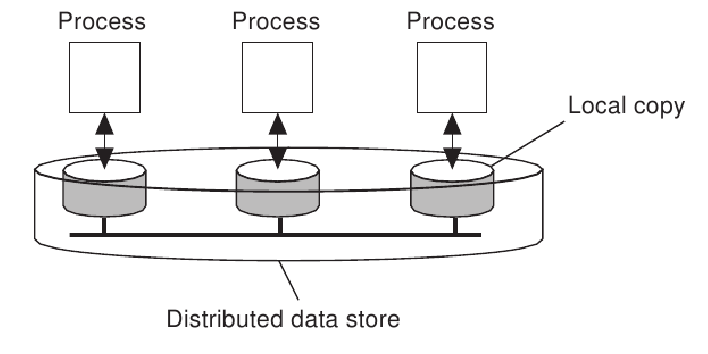
\includegraphics[width=\textwidth]{figs/09/datastore}
\end{figure}

\end{column}

\end{columns}

\end{frame}

%-------------------------------------------------------------------------
\begin{frame}{Consistency models}

\begin{block}{Werner Vogels}

\begin{columns}
\begin{column}{0.59\textwidth}
\begin{quote}
Whether or not inconsistencies are acceptable depends on the client application. 
In all cases \alert{the developer must be aware} that consistency guarantees
are provided by the storage systems and must be taken into account when
developing applications.
\end{quote}

{\footnotesize
\bibentry{eventual-consistent-nonote}
}
\end{column}
\begin{column}{0.39\textwidth}
\begin{figure}
	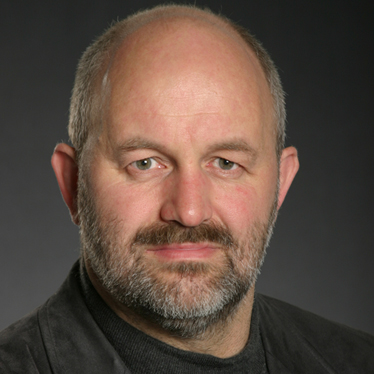
\includegraphics[width=0.8\textwidth]{figs/09/werner}
\end{figure}
Amazon's vice-president\\ and Chief Scientific Officer
\end{column}
\end{columns}

\end{block}


\end{frame}

%-------------------------------------------------------------------------
\begin{frame}{Consistency models}
	
\structure{Strong consistency models}
\BI
\item Strict consistency
\item Linearizability
\item Sequential consistency
\EI

\smallskip
\structure{Weak consistency models}
\BI
\item Eventual consistency
\item Client-centric consistency models
\BI
\item Read-after-read (monotonic read)
\item Read-after-write (read your writes)
% \item Write-after-write (monotonic write)
% \item Write-after-read (write follows read)	
\EI
\item Causal consistency 
\EI

\end{frame}	
	
%-------------------------------------------------------------------------
\begin{frame}{Notation}

\BIL
\item \alert{Write operation}: $w(x,v)$
\item \alert{Read operation}: $r(x) \rightarrow v$\\
\EIL

\begin{figure}
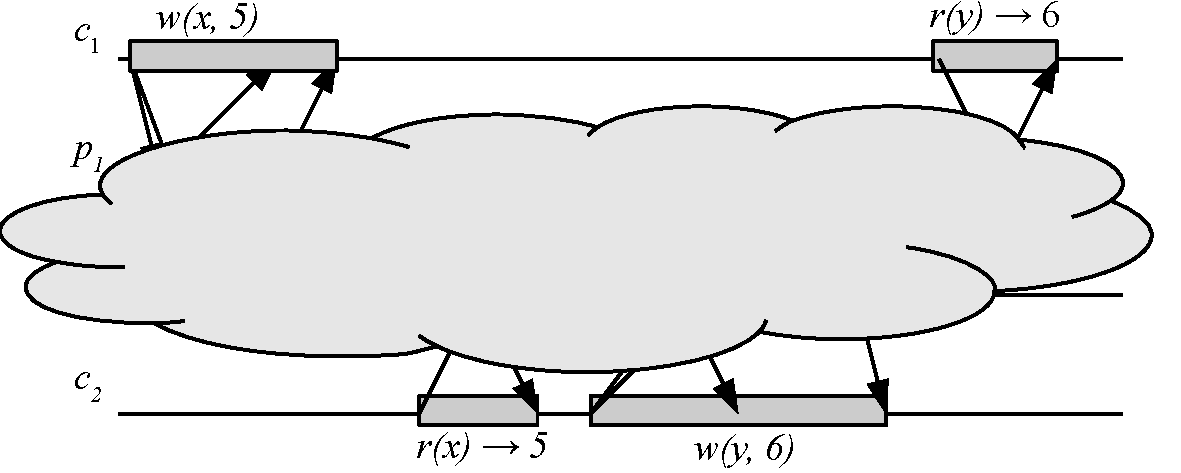
\includegraphics[width=\textwidth]{figs/09/lin-03}
\end{figure}

\end{frame}	

\subsection{Strong consistency models}


%%%%%%%%%%%%%%%%%%%%%%%%%%%%%%%%%%%%%%%%%%%%%%%%%%%%%%%%%%%%%%%%%%%%%%%%%%
\subsubsection{Strict consistency}

%-------------------------------------------------------------------------
\begin{frame}{Strict consistency}

\begin{definition}[Strict consistency]
A read operation must return the result of the latest write operation which occurred on the data item
\end{definition}

\smallskip
\structure{Implementation}:\\
\BI
\item Only possible with a global, perfectly synchronized clock
\item Only possible if all writes instantaneously visible to all
\EI

\smallskip
\structure{It makes sense, though}:\\
\BI
\item it is the model of uniprocessor systems!
\EI

\end{frame}

%%%%%%%%%%%%%%%%%%%%%%%%%%%%%%%%%%%%%%%%%%%%%%%%%%%%%%%%%%%%%%%%%%%%%%%%%%
\subsubsection{Linearizability}

%-------------------------------------------------------------------------
\begin{frame}[t]{Linearizability}

\begin{definition}[Linearizability, Herlihy and Wing, 1991]
An execution $E$ is linearizable provided that there exists a sequence (\alert{linearization}) $H$ such that
\BE
\item[L1] $H$ contains exactly the same operations that occur in $E$, each paired with the return value received in $E$
\item[L2] $H$ is a legal history of the sequential data type that is replicated
\item[L3] the total order of operations in $H$ is \alert{compatible} with the real-time partial order $<_{E,rt}$
\EE	
\end{definition}

\BI
\item $o_1 <_{E,rt} o_2$ means that the duration of operation $o_1$ (from invocation till it returns) occurs entirely before the duration of operation $o_2$
\item The \alert{real-time order} $<_{E,rt}$ is a partial order
\EI
\end{frame}

%-------------------------------------------------------------------------
\begin{frame}{Linearizability}

\begin{overprint}

\onslide<1|handout:1>
\begin{figure}
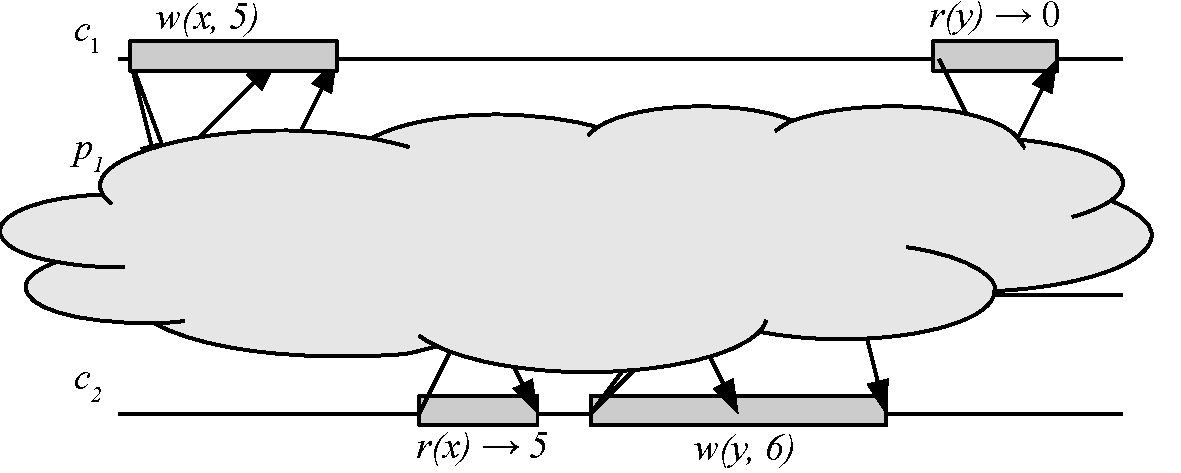
\includegraphics[width=0.7\textwidth]{figs/09/lin-01}
\end{figure}

\begin{example}
\BI
\item Are the following sequences possible linearizations?
\BI
\item $w(x,5) \quad r(x) \rightarrow 5 \quad w(y,6) \quad r(y) \rightarrow 0$
\item $w(x,5) \quad r(x) \rightarrow 5 \quad r(y) \rightarrow 0 \quad w(y,6)$
\EI
\item Is the above execution linearizable?\\ (Read: is there a sequence that is a linearization of the example?)
\EI
\end{example}

\onslide<2|handout:2>
\begin{figure}
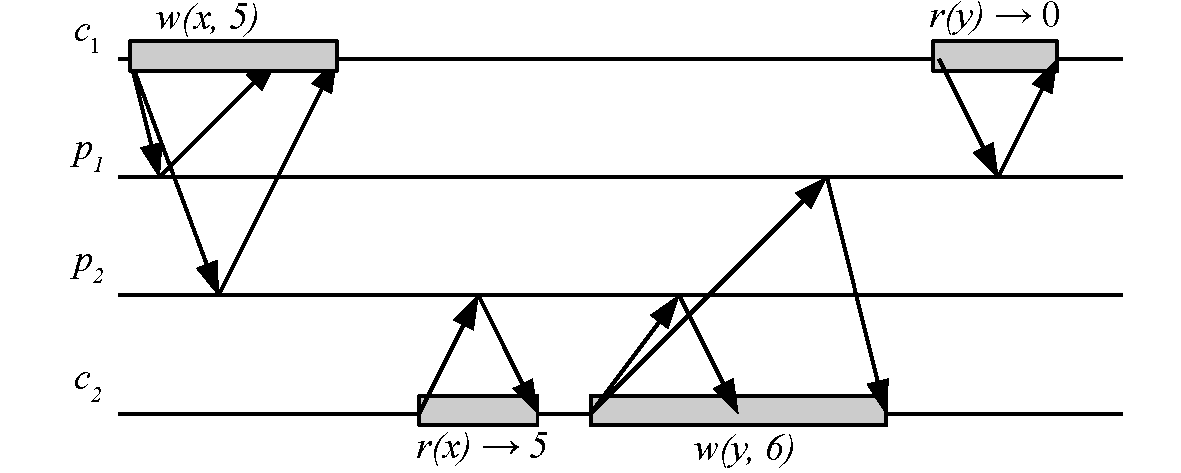
\includegraphics[width=0.7\textwidth]{figs/09/lin-01n}
\end{figure}

\begin{example}
\BI
\item Are the following sequences possible linearizations?
\BI
\item $w(x,5) \quad r(x) \rightarrow 5 \quad w(y,6) \quad r(y) \rightarrow 0$    \qquad NO!
\item $w(x,5) \quad r(x) \rightarrow 5 \quad r(y) \rightarrow 0 \quad w(y,6)$    \qquad NO!
\EI
\item Is the above execution linearizable?    \qquad NO! \\ (Read: is there a sequence that is a linearization of the example?) 
\EI
\end{example}

\end{overprint}

\end{frame}

%-------------------------------------------------------------------------
\begin{frame}{Linearizability}

\begin{overprint}
\onslide<1|handout:1>
\begin{figure}
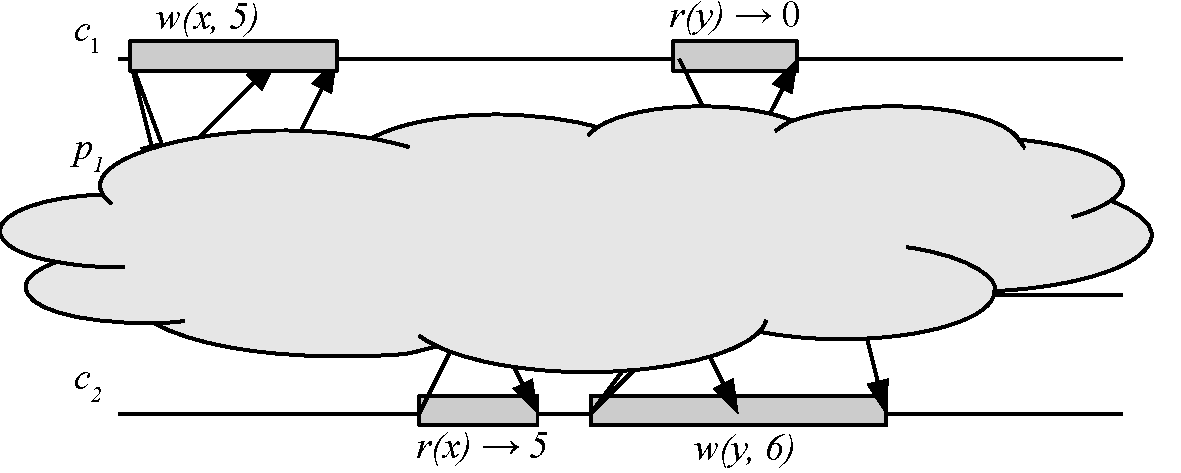
\includegraphics[width=0.7\textwidth]{figs/09/lin-02}
\end{figure}

\begin{example}
\BI
\item Are the following sequences possible linearizations?
\BI
\item $w(x,5) \quad r(x) \rightarrow 5 \quad w(y,6) \quad r(y) \rightarrow 0$
\item $w(x,5) \quad r(x) \rightarrow 5 \quad r(y) \rightarrow 0 \quad w(y,6)$
\EI
\item Is the above execution linearizable?\\ (Read: is there a sequence that is a linearization of the example?)
\EI
\end{example}

\onslide<2|handout:2>
\begin{figure}
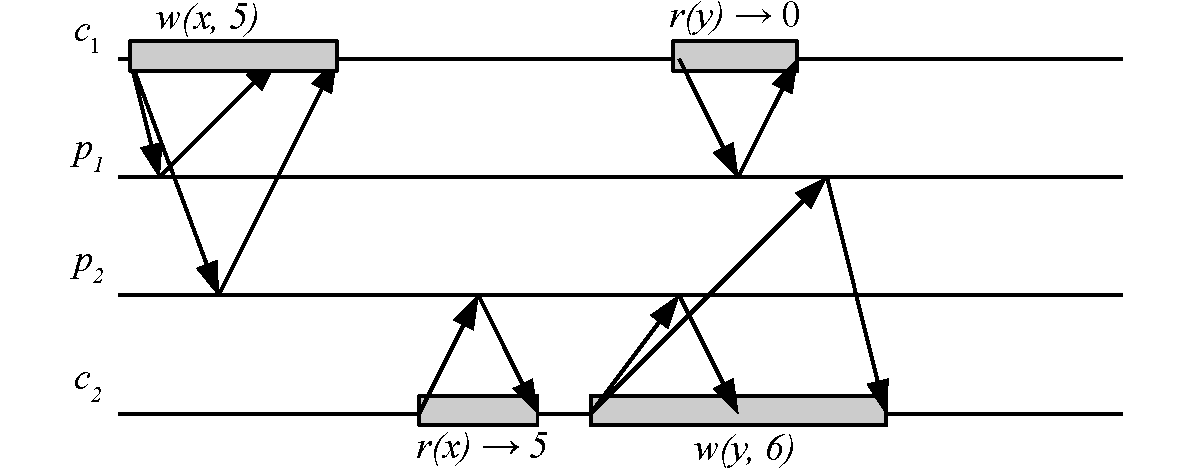
\includegraphics[width=0.7\textwidth]{figs/09/lin-02n}
\end{figure}

\begin{example}
\BI
\item Are the following sequences possible linearizations?
\BI
\item $w(x,5) \quad r(x) \rightarrow 5 \quad w(y,6) \quad r(y) \rightarrow 0$ \qquad NO!
\item $w(x,5) \quad r(x) \rightarrow 5 \quad r(y) \rightarrow 0 \quad w(y,6)$ \qquad YES!
\EI
\item Is the above execution linearizable? \qquad YES!\\ (Read: is there a sequence that is a linearization of the example?)
\EI

\end{example}

\end{overprint}

\end{frame}

%-------------------------------------------------------------------------
\begin{frame}{Linearizability}

\begin{overprint}
\onslide<1|handout:1>
\begin{figure}
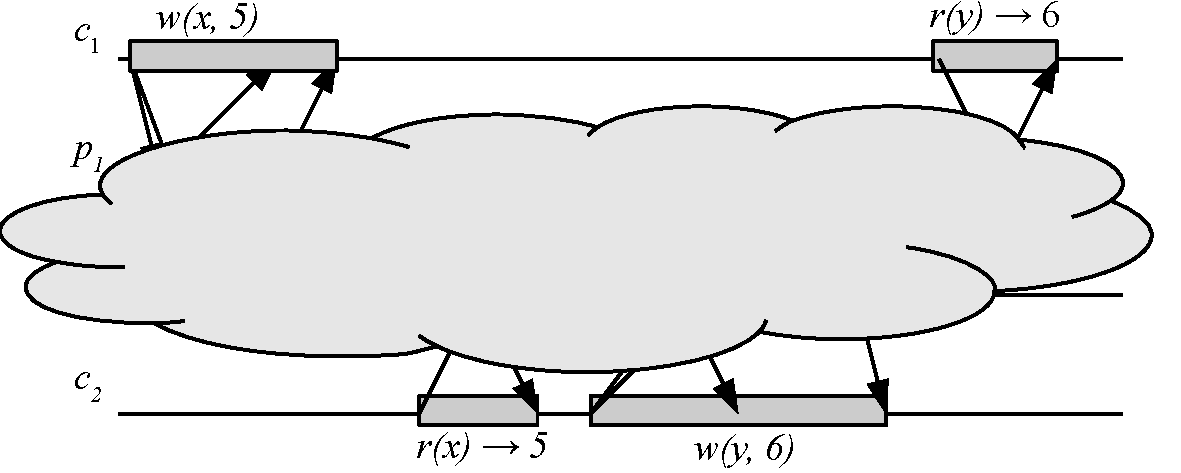
\includegraphics[width=0.7\textwidth]{figs/09/lin-03}
\end{figure}

\begin{example}
\BI
\item Are the following sequences possible linearizations?
\BI
\item $w(x,5) \quad r(x) \rightarrow 5 \quad w(y,6) \quad r(y) \rightarrow 6$
\item $w(x,5) \quad r(x) \rightarrow 5 \quad r(y) \rightarrow 6 \quad w(y,6)$
\EI
\item Is the above execution linearizable?\\ (Read: is there a sequence that is a linearization of the example?)
\EI
\end{example}

\onslide<2|handout:2>
\begin{figure}
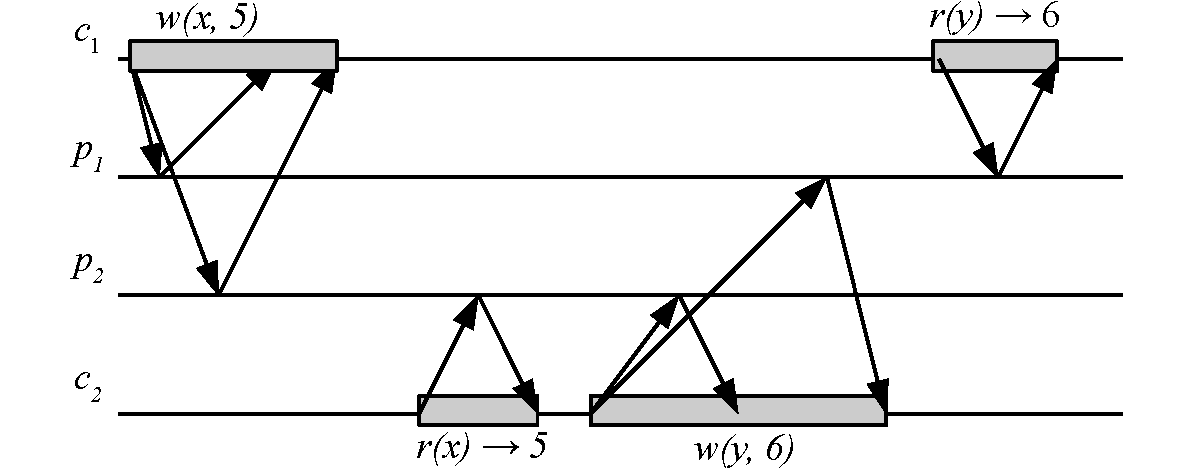
\includegraphics[width=0.7\textwidth]{figs/09/lin-03n}
\end{figure}

\begin{example}

\BI
\item Are the following sequences possible linearizations?
\BI
\item $w(x,5) \quad r(x) \rightarrow 5 \quad w(y,6) \quad r(y) \rightarrow 6$ \qquad YES!
\item $w(x,5) \quad r(x) \rightarrow 5 \quad r(y) \rightarrow 6 \quad w(y,6)$ \qquad NO!
\EI
\item Is the above execution linearizable? \qquad YES!\\ (Read: is there a sequence that is a linearization of the example?)
\EI
\end{example}

\end{overprint}
\end{frame}


%%%%%%%%%%%%%%%%%%%%%%%%%%%%%%%%%%%%%%%%%%%%%%%%%%%%%%%%%%%%%%%%%%%%%%%%%%
\subsubsection{Sequential consistency}

%-------------------------------------------------------------------------
\begin{frame}[t]{Sequential Consistency}

\begin{definition}[Sequential Consistency, Lamport, 1978]
An execution $E$ is sequential consistent provided that there exists a sequence $H$ such that
\BE	
\item[SC1] $H$ contains exactly the same operations that occur in $E$, each paired with the return value received in $E$
\item[SC2] $H$ is a legal history of the sequential data type that is replicated
\item[SC3] The total order of operations in $H$ is \alert{compatible} with the client partial order $<_{E,c}$
\EE	
\end{definition}

\BI
\item $o_1 <_{E,c} o_2$ means that the $o_1$ and $o_2$ occur at the same client and that $o_1$ returns before $o_2$ is invoked
\item The \alert{client order} $<_{E,c}$ is a partial order
\EI

\end{frame}


%-------------------------------------------------------------------------
\begin{frame}{Sequential Consistency}

\begin{overprint}

\onslide<1|handout:1>
\begin{figure}
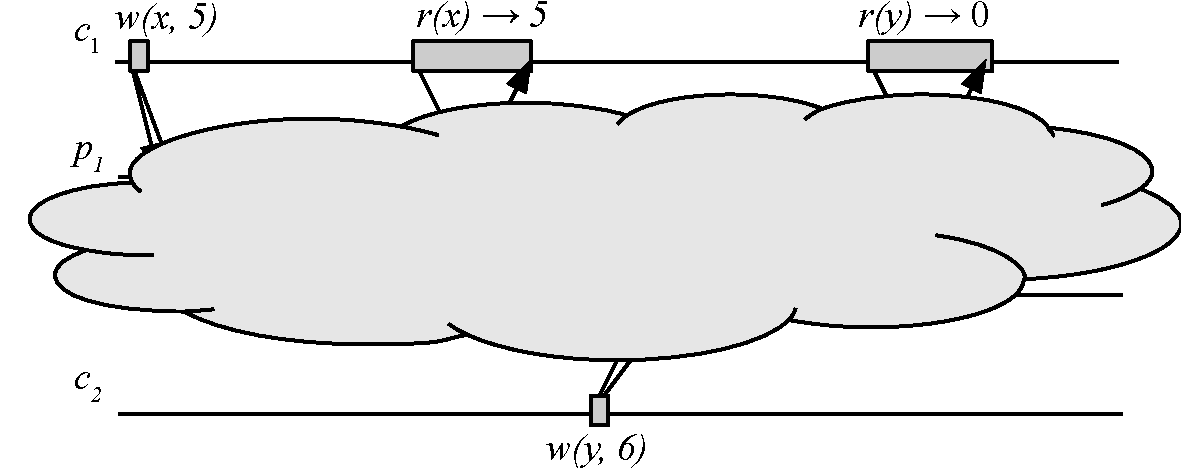
\includegraphics[width=0.7\textwidth]{figs/09/seq-01}
\end{figure}

\begin{example}

\BIL
\item Is the execution above sequentially consistent? 
\EIL

\end{example}

\onslide<2|handout:2>
\begin{figure}
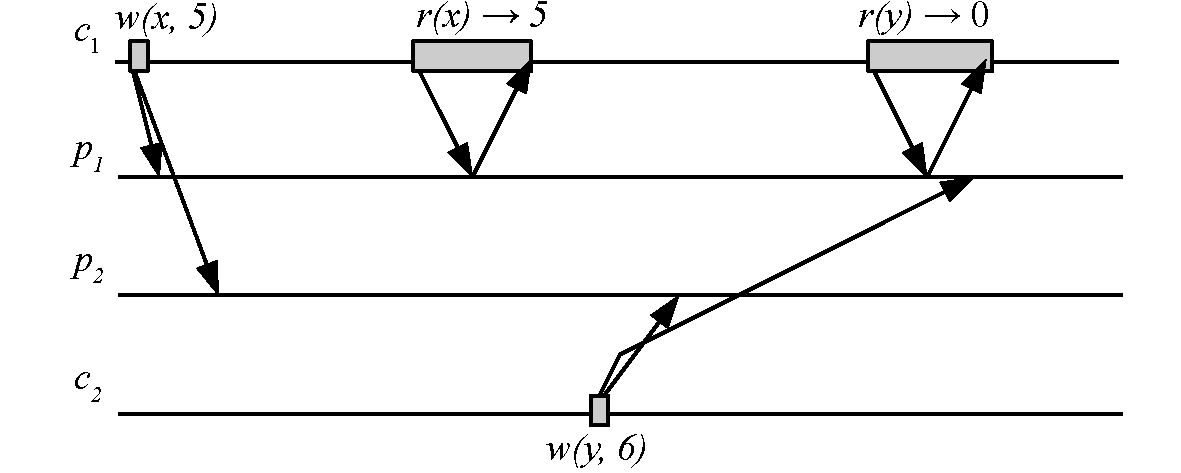
\includegraphics[width=0.7\textwidth]{figs/09/seq-01n}
\end{figure}

\begin{example}

\BIL
\item Is the execution above sequentially consistent? YES
\EIL

\end{example}

\end{overprint}

\end{frame}

%-------------------------------------------------------------------------
\begin{frame}{Sequential Consistency}

\begin{overprint}

\onslide<1|handout:1>
\begin{figure}
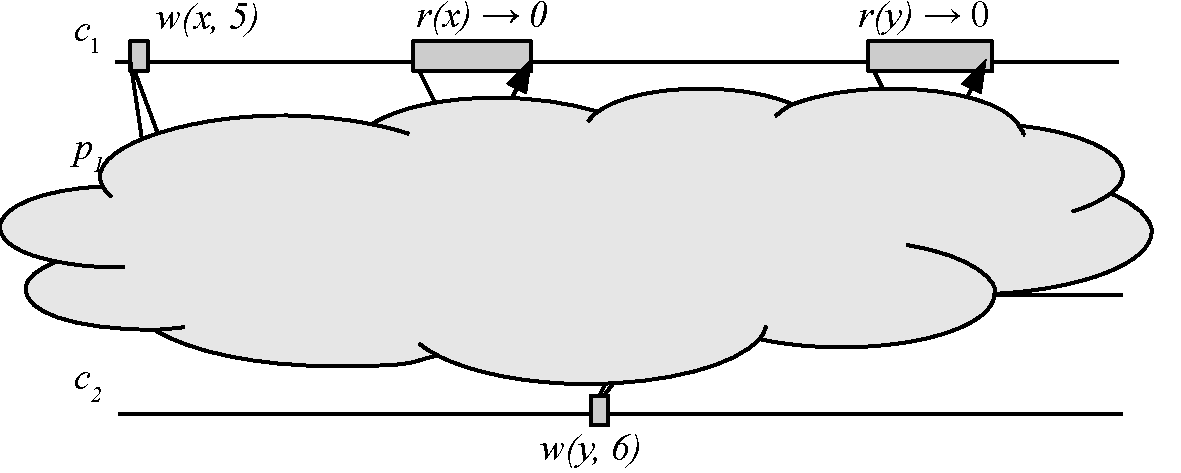
\includegraphics[width=0.7\textwidth]{figs/09/seq-02}
\end{figure}

\begin{example}

\BIL
\item Is the execution above sequentially consistent? 
\EIL

\end{example}

\onslide<2|handout:2>
\begin{figure}
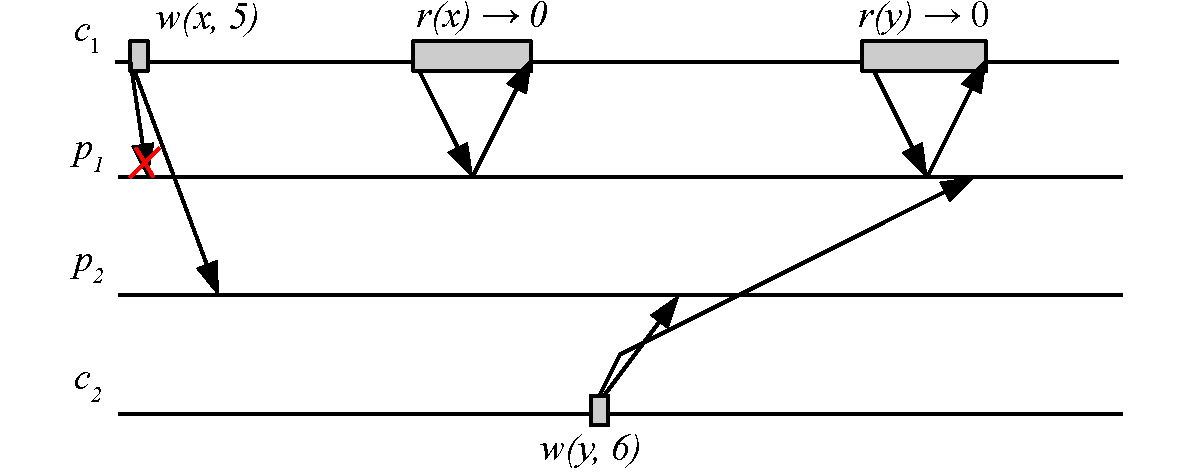
\includegraphics[width=0.7\textwidth]{figs/09/seq-02n}
\end{figure}

\begin{example}

\BIL
\item Is the execution above sequentially consistent? NO
\EIL

\end{example}

\end{overprint}

\end{frame}

%-------------------------------------------------------------------------
\begin{frame}{Sequential Consistency}

\begin{overprint}

\onslide<1|handout:1>
\begin{figure}
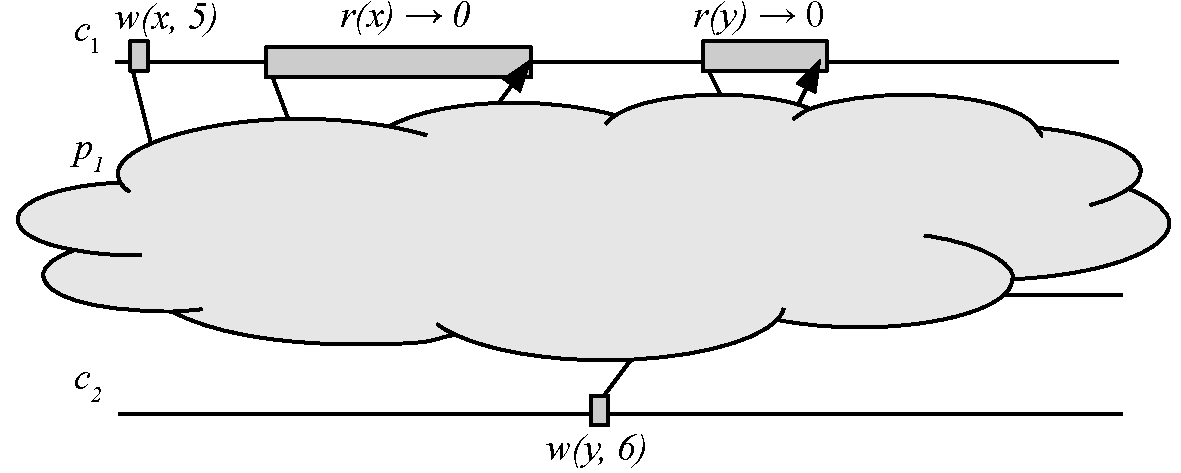
\includegraphics[width=0.7\textwidth]{figs/09/seq-03}
\end{figure}

\begin{example}

\BIL
\item Is the execution above sequentially consistent? 
\EIL

\end{example}

\onslide<2|handout:2>
\begin{figure}
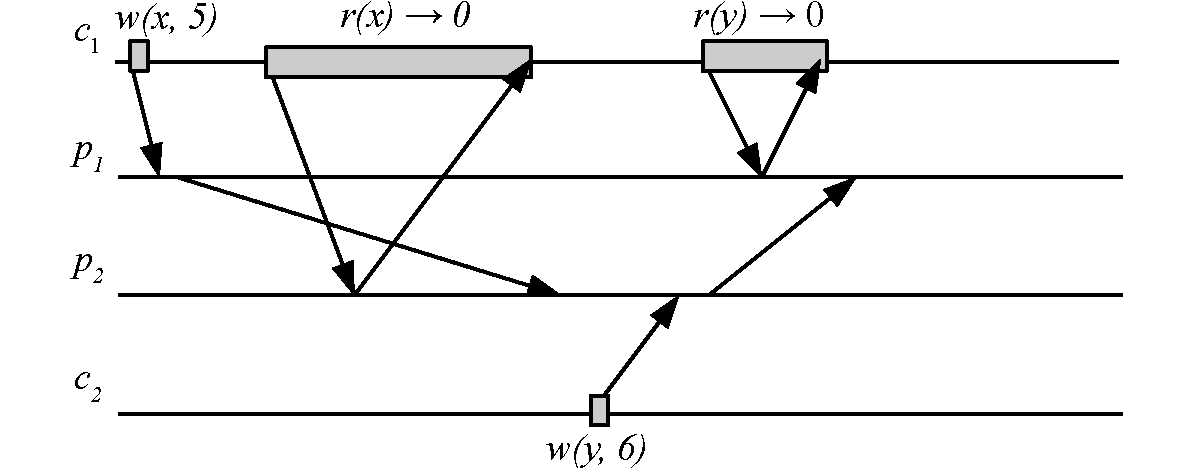
\includegraphics[width=0.7\textwidth]{figs/09/seq-03n}
\end{figure}

\begin{example}

\BIL
\item Is the execution above sequentially consistent? NO
\EIL

\end{example}

\end{overprint}

\end{frame}

%-------------------------------------------------------------------------
\begin{frame}{Sequential Consistency}

\begin{overprint}

\onslide<1|handout:1>
\begin{figure}
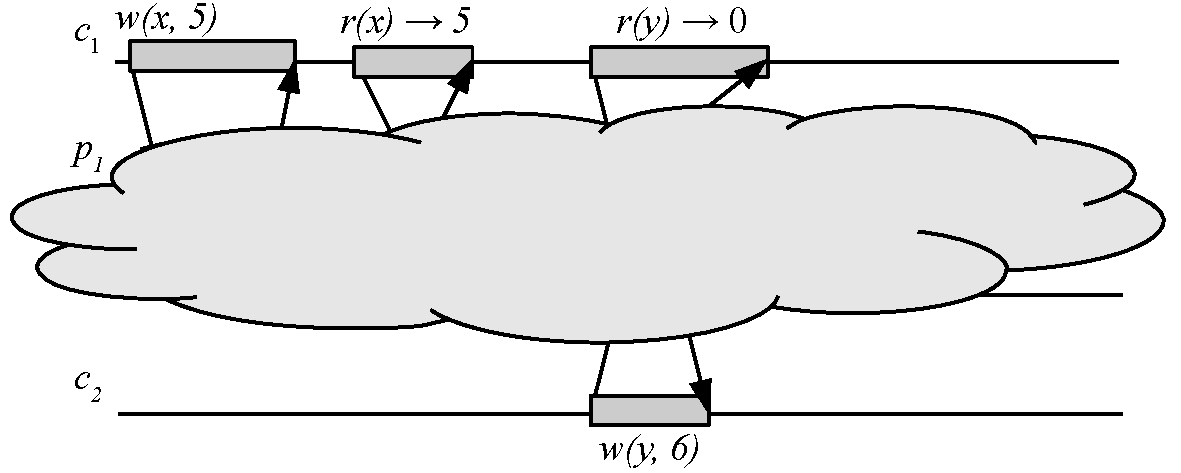
\includegraphics[width=0.7\textwidth]{figs/09/seq-04}
\end{figure}

\begin{example}

\BIL
\item Is the execution above sequentially consistent? 
\EIL

\end{example}

\onslide<2|handout:2>
\begin{figure}
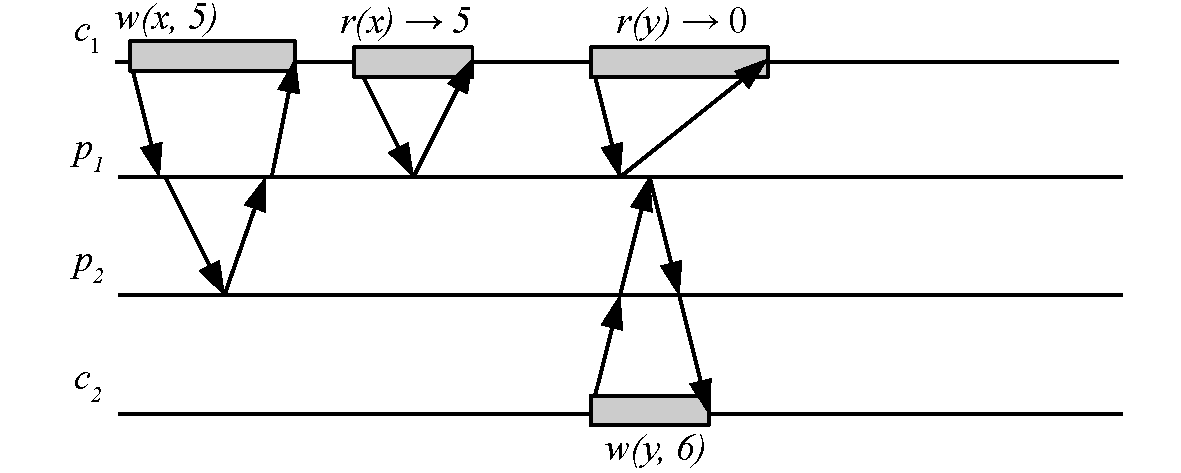
\includegraphics[width=0.7\textwidth]{figs/09/seq-04n}
\end{figure}

\begin{example}

\BIL
\item Is the execution above sequentially consistent? YES
\EIL

\end{example}

\end{overprint}

\end{frame}


%-------------------------------------------------------------------------
\begin{frame}{Sequential Consistency Example}
\begin{columns}
\begin{column}{0.30\textwidth}	
\begin{Procedure}
\caption{Process $p_1$}
$x \gets 1$\;
\PRINT $y,z$
\end{Procedure}
\end{column}
\hfill
\begin{column}{0.30\textwidth}	
\begin{Procedure}
\caption{Process $p_2$}
$y \gets 1$\;
\PRINT $x,z$
\end{Procedure}
\end{column}
\hfill
\begin{column}{0.30\textwidth}	
\begin{Procedure}
\caption{Process $p_3$}
$z \gets 1$\;
\PRINT $x,y$
\end{Procedure}
\end{column}	
\end{columns}

\bigskip
\BIL
\item Initially, all variables have value $0$

\item How many “potential executions” (actions executed in any order)?
\begin{overprint}
\onslide<1|handout:0>
~ 
\onslide<2-4|handout:1>
$6! = 720$
\end{overprint}
\item How many “valid executions” (with client partial order)?
\begin{overprint}
\onslide<1-2|handout:0>
~ 
\onslide<3-4|handout:1>
$(5!/4) \cdot 3 = 90$
\end{overprint}
\item How many “potential outputs” (signatures ordered by $p_1$, $p_2$, $p_3$)?
\begin{overprint}
\onslide<1-3|handout:0>
~ 
\onslide<4|handout:1>
$2^6 = 64$
\end{overprint}
\EIL

\note{
Three variables, replicated at the three processes. The $\rightarrow$ operation
is a write, the print operation require two reads.

\bigskip
\BIL
\item \alert{Potential executions}: corresponds top permutations, events can appear in any order
\item Valid executions: consider the $5! = 120$ possible execution sequences that start with $x \gets 1$
\BI
\item half of them have print $x,z$ before $y \gets 1$
\item half of this half have print $x,y$ before $z \gets 1$
\EI
so only $30$ out of $120$ respect condition $2$
\item If we consider the sequences that start with $y \gets 1$ and $z \gets 1$, we have $(5!/4) \cdot 3$
\EIL
}

\end{frame}

%-------------------------------------------------------------------------
\begin{frame}{Sequential Consistency}
\begin{columns}
\begin{column}{0.30\textwidth}	
\begin{Procedure}
\caption{Process $p_1$}
$x \gets 1$\;
\PRINT $y,z$
\end{Procedure}
\end{column}
\hfill
\begin{column}{0.30\textwidth}	
\begin{Procedure}
\caption{Process $p_2$}
$y \gets 1$\;
\PRINT $x,z$
\end{Procedure}
\end{column}
\hfill
\begin{column}{0.30\textwidth}	
\begin{Procedure}
\caption{Process $p_3$}
$z \gets 1$\;
\PRINT $x,y$
\end{Procedure}
\end{column}	
\end{columns}

\BIL	
\item How many “sequentially consistent outputs”? \pause $< 64$
\item  Example: Is 000000 sequentially consistent?  \pause No
	\BI
	\item All print operations “happen before” the updates - impossible
	\EI
\item Example: Is 001001 sequentially consistent? \pause No
\BI
\item print $yz=00$ after $x \gets 1$, before $y \gets 1$, $z \gets 1$
\item $x \gets 1$, \textbf{print} $yz=00$, $y \gets 1$, \textbf{print} $xz=10$, $z \gets 1$, \textbf{print} $xy=11$, No!
\item $x \gets 1$, \textbf{print} $yz=00$, $z \gets 1$ – no ($z$ was never equal to $1$)
\EI
\EIL

\end{frame}


%-------------------------------------------------------------------------
\begin{frame}{Several other models}
\BIL
\item FIFO/PRAM Consistency	(Lipton and Sandberg, 1988)
\item Release Consistency		(Gharachorloo et al, 1990)
\item Entry Consistency			(Bershad et al, 1993)
\item \ldots
\EIL
\end{frame}

%%%%%%%%%%%%%%%%%%%%%%%%%%%%%%%%%%%%%%%%%%%%%%%%%%%%%%%%%%%%%%%%%%%%%%%%%%
\subsection{Weak consistency models}

\begin{frame}{Weak consistency}

\begin{block}{Problem}
\BI	
\item It is easy to provide strong consistency through  appropriate hardware and/or software mechanisms
\item But these are typically found to incur considerable penalties, in latency, availability after faults, etc.
\EI
\end{block}

\begin{example}
\BI
\item Strong consistency often implies that message should arrive in the same order
\item Can be implemented through a sequencer replica
\item Latency: the sequencer replica becomes a bottleneck
\item Availability: a new sequencer must be elected after a failure
\EI
\end{example}

\end{frame}

\begin{frame}{Weak consistency}
	
\begin{block}{Weak consistency models}
Different weak models differs based by the precise details of
which reorderings are allowed
\BI
\item within the activity of a client
\item by whether there are any constraints at all on the
information provided to different clients
\EI
\end{block}

\end{frame}

\subsubsection{Eventual consistency}

%-------------------------------------------------------------------------
\begin{frame}{Eventual Consistency}
	
\structure{Scenario: consider a system where}

\BI
\item updates are rare
\item concurrent updates are absent, or can be easily resolved in an automatic way
\EI

\bigskip
\structure{Example: DNS}

\BI
\item Updates are rare w.r.t. to reads!
\item Only a centralized authority can update the system; no concurrent updates.
\EI

\bigskip
\structure{Do we need sequential consistency in this case?}

\end{frame}

%-------------------------------------------------------------------------
\begin{frame}{Eventual Consistency}

\begin{definition}[Eventual consistency]
If no updates take place for a long time, all replicas will gradually become consistent (i.e., the same)
\end{definition}

\bigskip
\structure{Comment}:

\BIL
\item The consistency policy of epidemic protocols
\item This is not a safety property, is a liveness one
\item What happens in our three- process example with prints?
\EIL

\end{frame}

%-------------------------------------------------------------------------
\begin{frame}{Eventual Consistency}
\begin{columns}
\begin{column}{0.30\textwidth}	
\begin{Procedure}
\caption{Process $p_1$}
$x \gets 1$\;
\PRINT $y,z$
\end{Procedure}
\end{column}
\hfill
\begin{column}{0.30\textwidth}	
\begin{Procedure}
\caption{Process $p_2$}
$y \gets 1$\;
\PRINT $x,z$
\end{Procedure}
\end{column}
\hfill
\begin{column}{0.30\textwidth}	
\begin{Procedure}
\caption{Process $p_3$}
$z \gets 1$\;
\PRINT $x,y$
\end{Procedure}
\end{column}	
\end{columns}

\BIL	
\item Example: Is 000000 eventual consistent?  \pause Yes
\item In general, all the potential 64 outputs are possible
\EIL

\end{frame}

\subsubsection{Client-centric consistency}

%-------------------------------------------------------------------------
\begin{frame}{Consistency for mobile users}

Consider a replicated database that you access through your notebook. 
The notebook acts as a front-end to the database

\begin{figure}
	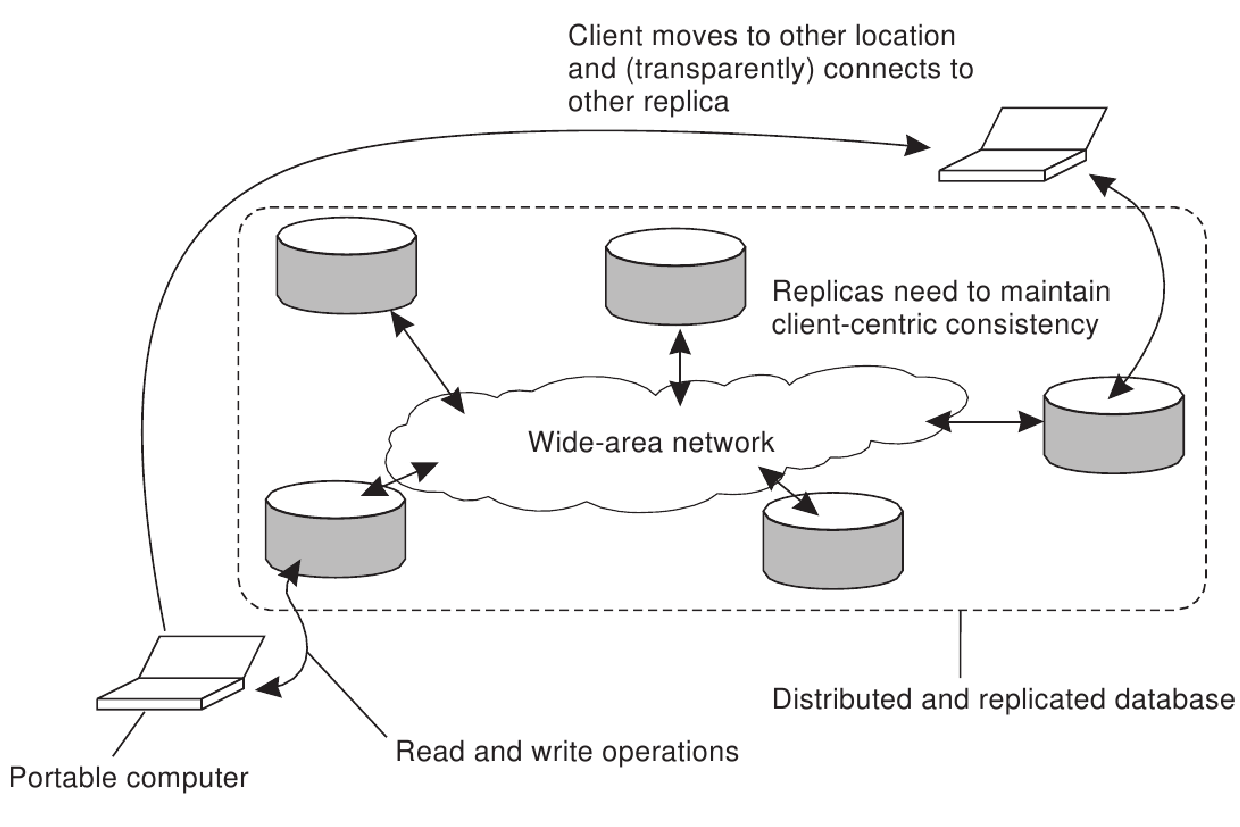
\includegraphics[width=0.8\textwidth]{figs/09/mobile}
\end{figure}

\end{frame}

%%%%%%%%%%%%%%%%%%%%%%%%%%%%%%%%%%%%%%%%%%%%%%%%%%%%%%%%%%%%%%%%%%%%%%%%%%

%-------------------------------------------------------------------------
\begin{frame}{Consistency for mobile users}
\begin{block}{Problem: Eventual Consistency is not sufficient}
\BI
\item You move from location $A$ to location $B$
\item Unless you use the same server, you may detect inconsistencies:
\BI
\item your updates at $A$ may not have yet been propagated to $B$
\item you may be reading newer entries than the ones available at $A$
\item your updates at $B$ may eventually conflict with those at $A$
\EI
\EI
\end{block}

\bigskip
\structure{What we can do?}

The only thing you really care is that the entries you updated and/or read at
$A$, are in $B$ the way you left them in $A$. In that case, the database will
appear to be consistent to \alert{you}
\end{frame}

%-------------------------------------------------------------------------
\begin{frame}{Client-centric consistency}

\begin{block}{Idea}
In some cases, we can avoid system-wide consistency, by concentrating on what
specific clients want, instead of what should be provided by servers
\end{block}

\bigskip
\structure{Models}:
\BI
\item Read-after-read / Monotonic reads
\item Write-after-write / Monotonic writes
\item Read-after-write / Read-your-writes
\item Write-after-read / Write-follows-reads
\EI

\end{frame}

\begin{frame}{Justifications}
\begin{definition}[Justification]
Each operation $o$ performed in an execution $E$ has a \alert{justification}
$J_o$, which is a sequence of other operations that occurred in $E$ such
that the return value $o$ received in $E$ is the one which the sequential data type would 
give to operation $o$ when performed in the state which is produced
by starting in the initial state and then applying each operation in $J_o$ in
turn.
\end{definition}
\end{frame}



% %-------------------------------------------------------------------------
% \begin{frame}{Notation}
% \BIL
% \item $x_i$ denotes the version of data item $x$ at local copy $L_i$ 
% \item $\mathit{WS}(x_i)$ denotes the set of the write/update operations that
%   have caused $x_i$ to assume such value on $L_i$
% \item $\mathit{WS}(x_i;x_j)$ denotes the fact that the operations in $\mathit{WS}(x_i)$ have
% been also performed at local copy $L_j$
% \item Time specifications should be added to this notation; in the next
% slides we will use a space-time diagram, instead
% \EIL
% \end{frame}

%-------------------------------------------------------------------------
\begin{frame}{Monotonic reads -- Read-after-read}

\begin{definition}[Monotonic reads]
If a process reads data item $x$, any successive read operation 
on $x$ by that process will always return that same value or a more recent one
\vspace{-12pt}
\begin{center}
\begin{minipage}{0.95\textwidth}
\begin{block}{Formally}
Given two read operations $o_1$ and $o_2$ submitted by a client $c$, the
justification $J_{o_1}$ is a prefix of justification of $J_{o_2}$
\end{block}
\end{minipage}
\end{center}
\end{definition}

% \begin{columns}
% \begin{column}{0.45\textwidth}
\begin{example}
Reading incoming mail on a web-server. Each time you connect to a different 
e-mail server, that server fetches (at least) all the updates from the 
server you previously visited
\end{example}
% \end{column}
% \hfill
% \begin{column}{0.50\textwidth}
% 
% \end{column}
% \end{columns}

\end{frame}

%-------------------------------------------------------------------------
\begin{frame}{Monotonic reads -- Read-after-read}

\begin{overprint}
\onslide<1|handout:1>
\begin{figure}
	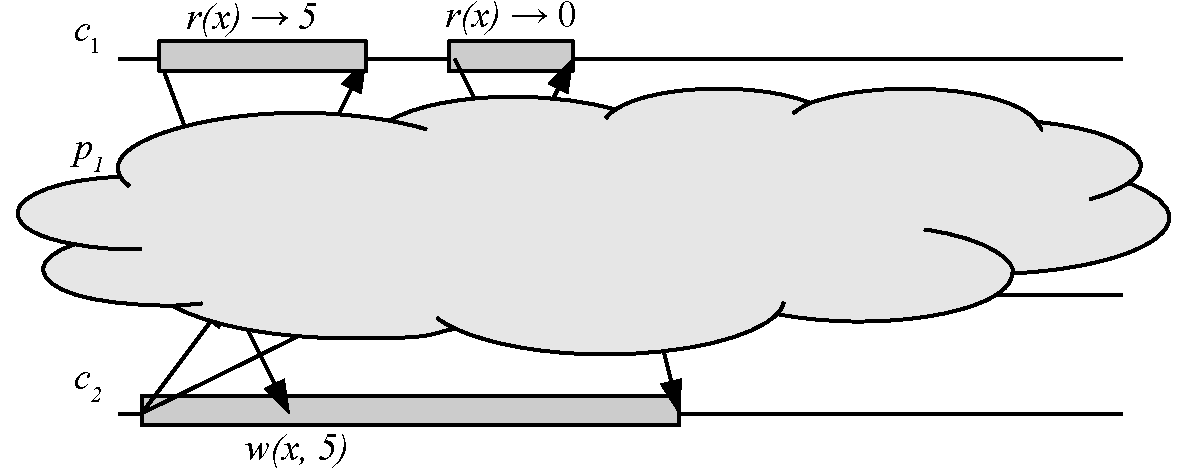
\includegraphics[width=\textwidth]{figs/09/read-after-read-01}
\end{figure}
\BI
\item Is the above execution satisfying read-after-read?
\EI
\onslide<2|handout:2>
\begin{figure}
	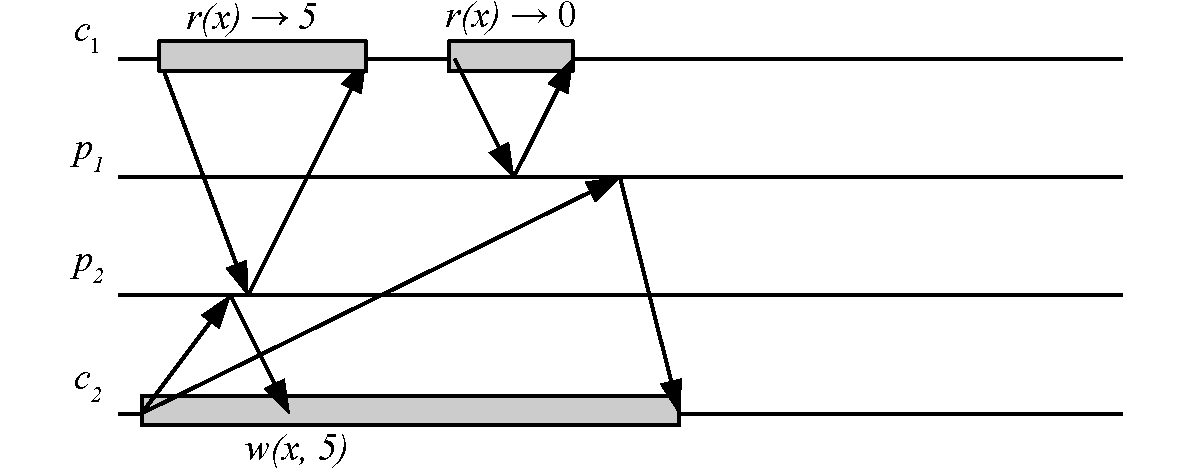
\includegraphics[width=\textwidth]{figs/09/read-after-read-01n}
\end{figure}
\BI
\item Is the above execution satisfying read-after-read? \quad NO!
\EI
\onslide<3|handout:3>
\begin{figure}
	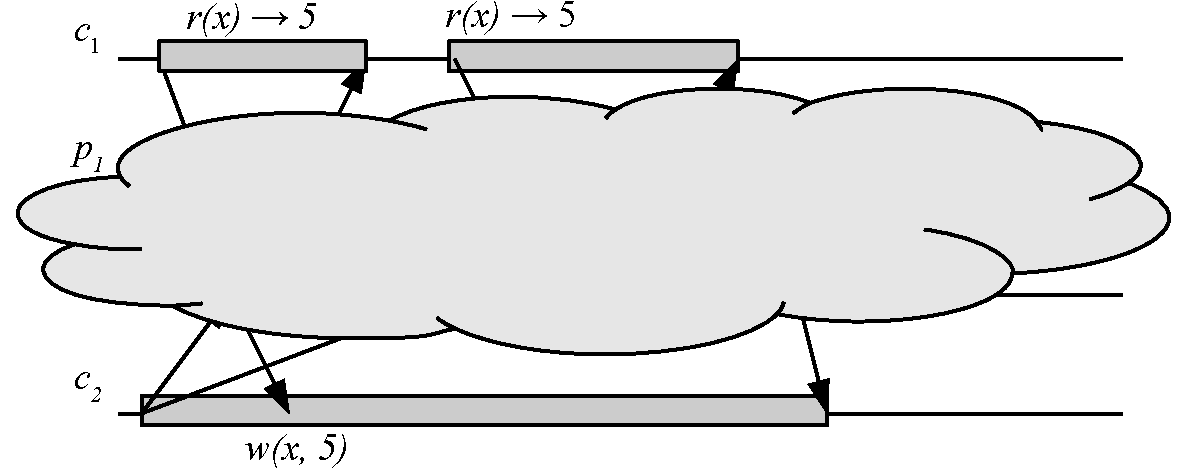
\includegraphics[width=\textwidth]{figs/09/read-after-read-02}
\end{figure}
\BI
\item Is the above execution satisfying read-after-read?
\EI
\onslide<4|handout:4>
\begin{figure}
	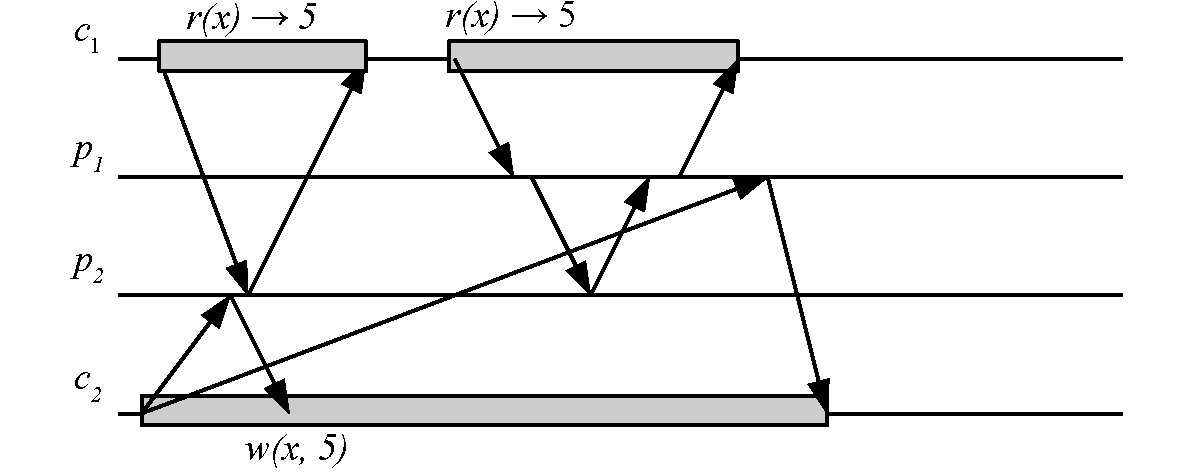
\includegraphics[width=\textwidth]{figs/09/read-after-read-02n}
\end{figure}
\BI
\item Is the above execution satisfying read-after-read? \quad YES!
\EI

\end{overprint}
\end{frame}


%-------------------------------------------------------------------------
\begin{frame}{Read your writes -- Read-after-write}

\begin{definition}[Read your writes]
The effect of a write operation by a process on data item $x$, will always 
be seen by a successive read operation on $x$ by the same process
\vspace{-12pt}
\begin{center}
\begin{minipage}{0.95\textwidth}
\begin{block}{Formally}
When submitting a read operation $o$,
$J_o$ is equal to  the sequence of write operation performed by client $c$ before
submitting $o$.
\end{block}
\end{minipage}
\end{center}
\end{definition}

% \begin{columns}
% \begin{column}{0.45\textwidth}
\begin{example}
Updating your web page and guaranteeing that your web browser shows the
newest version instead of its cached copy
\end{example}
% \end{column}
% \hfill
% \begin{column}{0.50\textwidth}
% 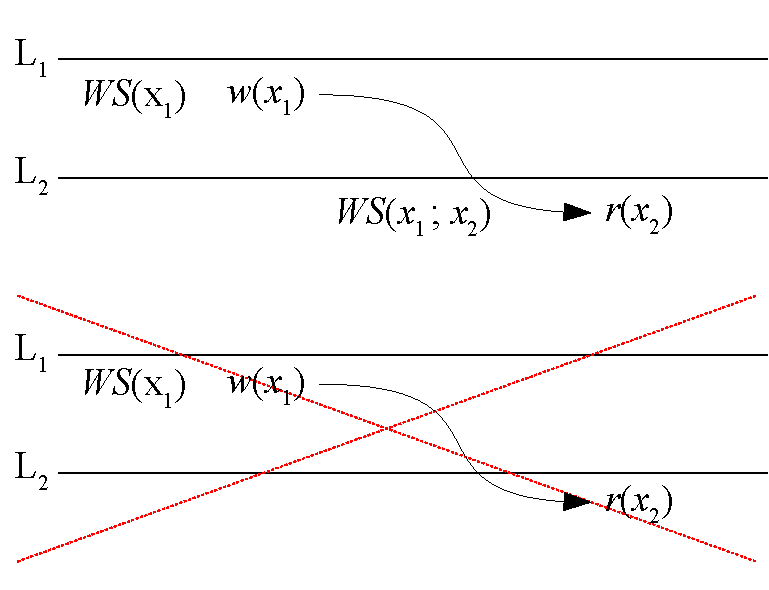
\includegraphics[width=\textwidth]{figs/09/readyourwrites}
% \end{column}
% \end{columns}

\end{frame}

%-------------------------------------------------------------------------
\begin{frame}{Other client-centric models}

\begin{definition}[Monotonic writes]
A write operation by a process on a data item $x$ is completed before any
successive write operation on $x$ by the same process
\end{definition}

% \begin{columns}
% \begin{column}{0.45\textwidth}
% \begin{example}
% Maintaining versions of replicated files in the correct order everywhere
% (propagate the previous version to the server where the newest version is installed)
% \end{example}
% \end{column}
% \hfill
% \begin{column}{0.50\textwidth}
% 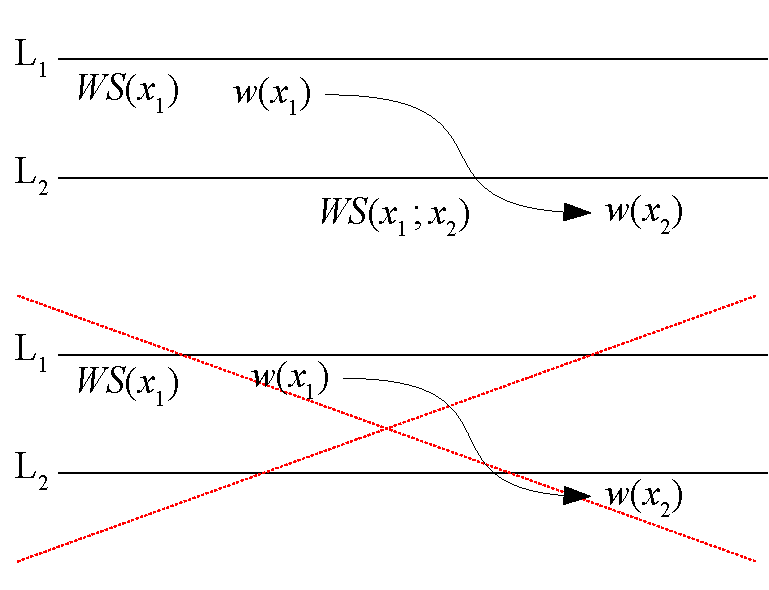
\includegraphics[width=\textwidth]{figs/09/writewrite}
% \end{column}
% \end{columns}

% \end{frame}
% 
% 
% 
% %-------------------------------------------------------------------------
% \begin{frame}{Writes follow read -- Write-after-read}

\begin{definition}[Writes follow read]
A write operation by a process $P$ on a data item $x$ following a previous 
read operation on $x$ by $P$, is guaranteed to take place on the same or a 
more recent value of $x$ that was read
\end{definition}

% \begin{columns}
% \begin{column}{0.45\textwidth}
% \begin{example}[Newsgroup]
% To guarantee that users of a network newsgroup see a posting of a reaction
% to an article only after they have seen the original article
% \end{example}
% \end{column}
% \hfill
% \begin{column}{0.50\textwidth}
% 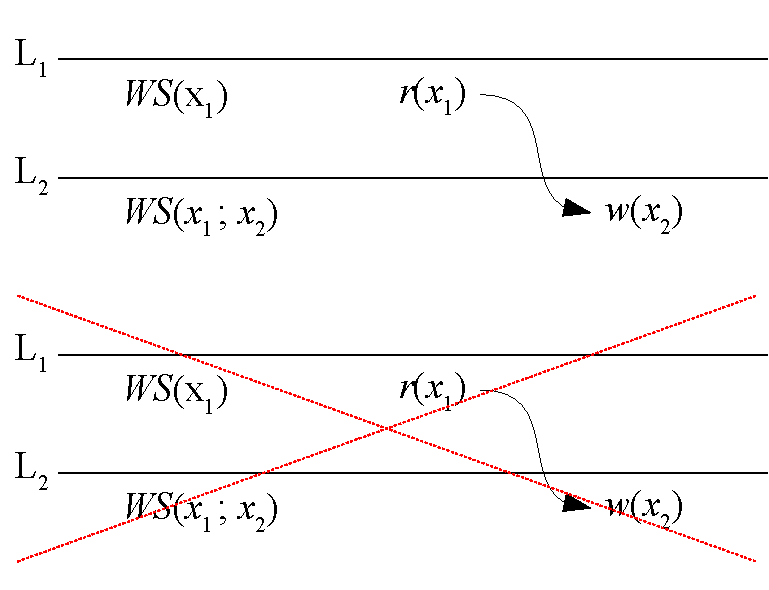
\includegraphics[width=\textwidth]{figs/09/writefollowread}
% \end{column}
% \end{columns}

\note{
\BI
\item To understand the problem, assume that a user first reads an article $A$.
\item Then, he reacts by posting a response $B$
\item By requiring writes-follow-reads consistency, $B$, will be written
to any copy of the newsgroup only after $A$ has been written as well.
\EI

\bigskip
Causal consistency wouldn't be better in this case?
}

\end{frame}

%-------------------------------------------------------------------------
\begin{frame}{Session consistency}

\begin{definition}[Session consistency]
\BIL
\item A practical version of read-your-writes, where processes access a data storage
in the context of a session
\item As long as the session exists, the system guarantees read-your-writes
\item If the session terminates because of a failure, a new session must be
created
\item Guarantees are limited to sessions
\EIL
\end{definition}

\end{frame}

%-------------------------------------------------------------------------
\begin{frame}{Causal Consistency -- (Hutto and Ahamad, 1990)}

\begin{definition}[Causal Consistency]	
All writes that are (potentially) causally related must be seen by every process in causal order
\end{definition}

\bigskip
\structure{Define “causally related”}:

\BIL
\item a read followed by a write, on the same process: 
	\BI
	\item the write is (potentially) causally related by the read
	\EI
\item a write followed by a read of the same value, on diff. process: 
	\BI
	\item the read is (potentially) causally related by the write
	\EI
\EIL

\bigskip
\structure{Example of use}:
\BI
\item Bulletin board
\EI

\end{frame}

%-------------------------------------------------------------------------
\begin{frame}{Causal Consistency}
	
\begin{example}
\BI
\item Is the following example causally consistent? \only<2-3|handout:0>{Yes!}
\item Is the following example sequentially consistent?	\only<3|handout:0>{No!}
\EI
\end{example}	
	
\begin{figure}
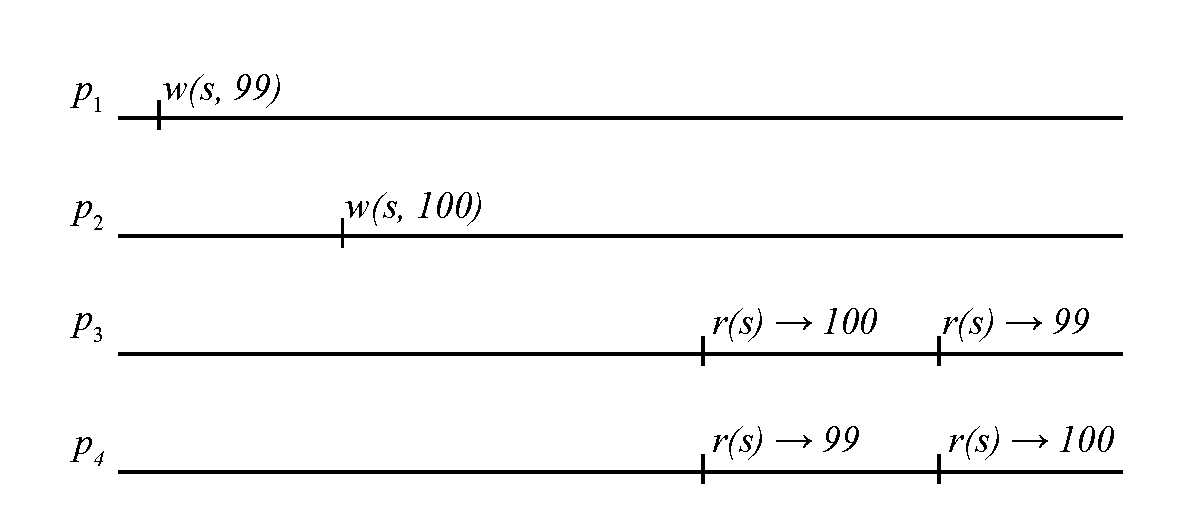
\includegraphics[width=\textwidth]{figs/09/scenario3}
\end{figure}

\note{Interpretation: message 99 and message 100 are written in a newsgroup. 
Given that the two messages are not related, they could appear in any order.}

\end{frame}

%-------------------------------------------------------------------------
\begin{frame}{Causal Consistency}
	
\begin{example}
\BI
\item Is the following example causally consistent? \only<2-3|handout:0>{No!}
\item Is the following example sequentially consistent?	\only<3|handout:0>{Yes!}
\EI
\end{example}	
	
\begin{figure}
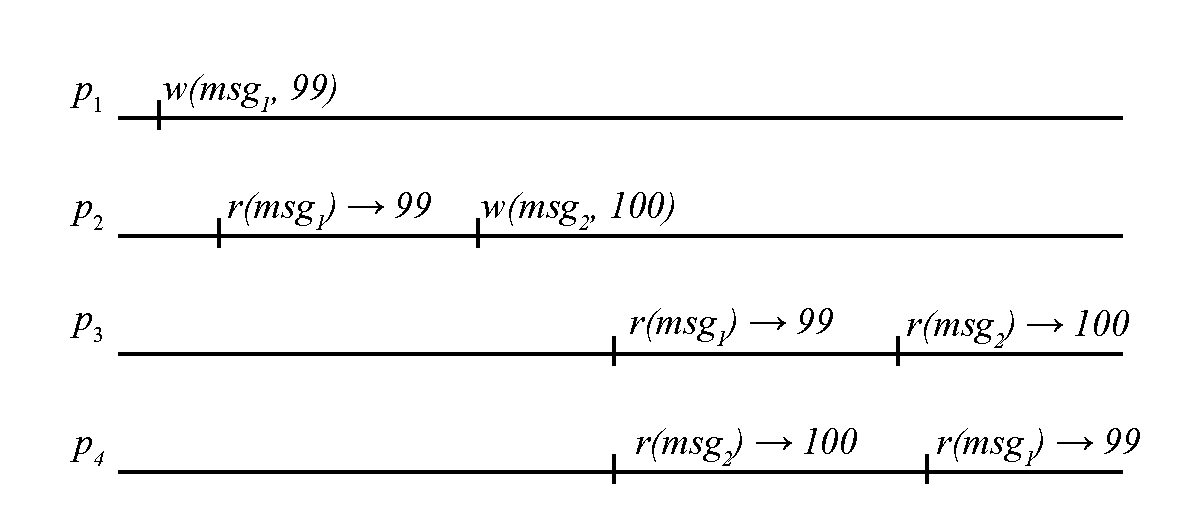
\includegraphics[width=\textwidth]{figs/09/scenario4}
\end{figure}

\note{Interpretation: message 99 and message 100 are written in a newsgroup. Message 100 could be potentially
caused by message 99}

\end{frame}



%-------------------------------------------------------------------------
\begin{frame}{Reality Check}

\begin{block}{Amazon S3}
Amazon S3 (Simple Storage Service) is an online storage web service offered by Amazon Web Services.
S3 is designed to provide   99.99\% availability and 99.999999999\% durability of objects over a given year.
\end{block}

\smallskip
\begin{block}{From Amazon S3's FAQ}
\begin{quote}
\textbf{Q}: \underline{What data consistency model does Amazon S3 employ}?
Amazon S3 buckets in the US West (Northern California), EU (Ireland), Asia
Pacific (Singapore), and Asia Pacific (Tokyo) Regions provide
\alert{read-after-write} consistency for PUTS of new objects and
\alert{eventual consistency} for overwrite PUTS and DELETES. Amazon S3 buckets
in the US Standard Region provide \alert{eventual
consistency}.
\end{quote}
\end{block}

\end{frame}

%-------------------------------------------------------------------------
\begin{frame}{Reality Check}

\begin{block}{Berkeley DB}
Oracle's Berkeley DB is a computer software library that provides a 
high-performance embedded database for key/value data. Used in Postfix,
Subversion, SpamAssassin, BitCoin.
\end{block}

\smallskip
\begin{block}{From the Berkeley DB manual}
\begin{quote}
In a distributed system, the changes made at the master are not always
instantaneously available at every replica, although they \alert{eventually}
will be. In general, replicas not directly involved in contributing to a
transaction commit will lag behind other replicas because they do not
synchronize their commits with the master. For this reason, you might want to
make use of the \alert{read-your-writes} consistency feature.
\end{quote}
\end{block}

\end{frame}

%-------------------------------------------------------------------------
\begin{frame}{Reality Check}

\begin{block}{Apache ZooKeeper}
Apache ZooKeeper is a software project of the Apache Software Foundation,
providing an open source centralized configuration service and naming registry
for large distributed systems. ZooKeeper is a sub project of Hadoop.
\end{block}

\smallskip
\begin{block}{From ZooKeeper}
\begin{quote}
\alert{Sequential Consistency}: Updates from a client will be applied in the order that they were sent.
\end{quote}
\end{block}

\bigskip
What?

\end{frame}

%-------------------------------------------------------------------------
\begin{frame}{Reading material}

\begin{Bib}
{\footnotesize
\BIL
\item \bibentry{Replication}
\EIL
}
\end{Bib}

% \invisible{{\tiny
% \bibliographystyle{abbrv}
% \bibliography{../references} 
% }}

\end{frame}

%-------------------------------------------------------------------------
\begin{frame}{Additional readings}

\begin{Bib}
{\footnotesize
\BI
\item \alert{\bibentry{cloud-consistency}}
\item \bibentry{bayou}
\item \bibentry{tvs}. [Chapter 7]
\EI
}
\end{Bib}

% \invisible{{\tiny
% \bibliographystyle{abbrv}
% \bibliography{../references} 
% }}

\end{frame}



%%%%%%%%%%%%%%%%%%%%%%%%%%%%%%%%%%%%%%%%%%%%%%%%%%%%%%%%%%%%%%%%%%%%%%%%%%
\section{Replication architectures}

\subsection{Overview}


%-------------------------------------------------------------------------
\begin{frame}{Passive replication}
\BI
\item Clients communicate with primary server
\item Updates are forwarded from primary to backups
\item Queries are replied by the primary	
\EI

\begin{figure}
	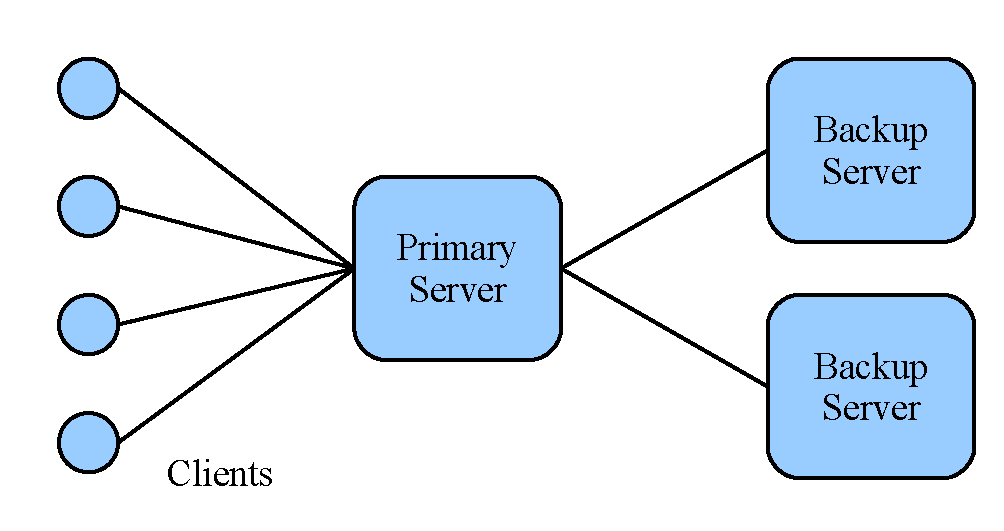
\includegraphics[width=0.8\textwidth]{figs/09/primarybackup}
\end{figure}

\end{frame}

%-------------------------------------------------------------------------
\begin{frame}{Active replication}
\BI
\item Several (all) replicas handle the invocation and send the response
\item Updates must be applied in the same order – total order broadcast 
\EI
\begin{figure}
	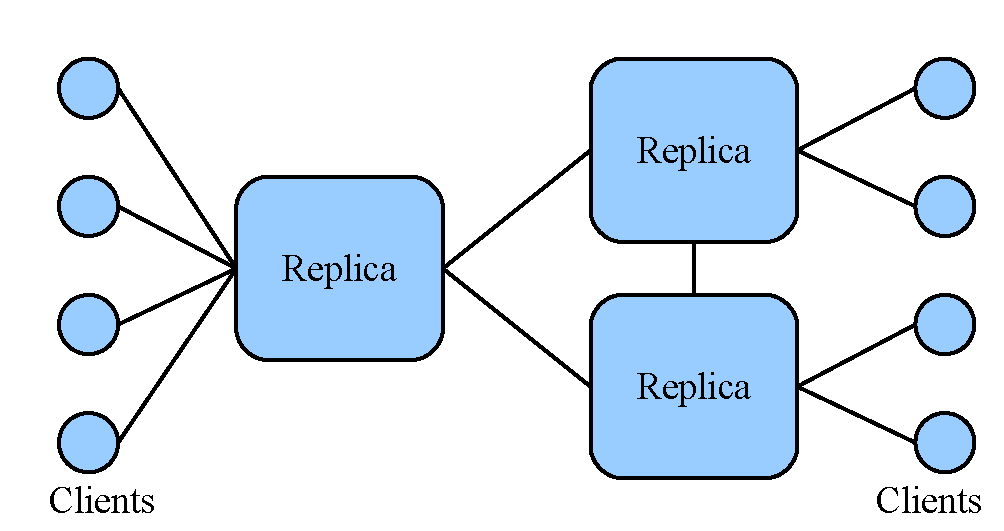
\includegraphics[width=0.8\textwidth]{figs/09/active}
\end{figure}

\end{frame}

%-------------------------------------------------------------------------
\begin{frame}{Passive vs Active}

\structure{Passive replication}\\
\BI
\item Computation is performed only at primary
\item If state updates are large, can waste network bandwidth
\item Can handle non-determinism
\EI

\bigskip
\structure{Active replication}\\
\BI
\item Small recovery delay after failures
\item If operations are compute intensive, can waste computational resources
\item Only deterministic
\EI

\end{frame}


%-------------------------------------------------------------------------
\begin{frame}{Consistency protocols}

\BIL
\item Primary-based protocols
	\BI
	\item Definition
	\item Lower bounds
	\EI
\item Replicated-write protocols
	\BI
	\item Majority, quorum-based
	\item State machine approach
	\EI
\item Client-centric protocols
\BI
\item Monotonic reads
\item Read-your-writes
\EI
\EIL

\end{frame}

%%%%%%%%%%%%%%%%%%%%%%%%%%%%%%%%%%%%%%%%%%%%%%%%%%%%%%%%%%%%%%%%%%%%%%%%%%
\subsection{Primary-Backup}

%-------------------------------------------------------------------------
\begin{frame}{Primary-Backup}

\begin{block}{The idea}
\BIL
\item Clients communicate with a single replica (the \alert{primary})
\item The primary updates the other replicas (\alert{backup})
\item Backups detect the failure of the primary using a timeout mechanism
\item Clients learn from the service when the primary fails and the service “fail over” to a backup
\item Note: non-deterministic events are executed only at the primary
\EIL
\end{block}

\end{frame}

%-------------------------------------------------------------------------
\begin{frame}{How to evaluate a primary-backup protocol}

\begin{definition}[Degree of replication]
Number of servers used to implement the service; the smaller, the better
\end{definition}

\bigskip
\begin{definition}[Blocking time]
The worst-case period between a request and its response in any failure-free execution
\end{definition}

\bigskip
\begin{definition}[Failover time]
The worst-case period during which request can be lost because there is no primary
\end{definition}

\end{frame}

%-------------------------------------------------------------------------
\begin{frame}{Definitions}

\begin{definition}[Service outage]
The service has a server outage at $t$ if some correct client sends a request
at time $t$ to the service, but does not receive a response
\end{definition}

\bigskip
\begin{definition}[$(k, \Delta)$-bofo service - “bounded outage, finitely often”]
A service in which all server outages can be grouped into at most $k$
intervals of time, each of them at most length $\Delta$
\end{definition}

\end{frame}

%-------------------------------------------------------------------------
\begin{frame}{Specification}
\BIL
\item[PB1] At any time, there is \alert{at most} one server $p_i$ that acts as
a primary
\item[PB2] If a client request arrives at a server that is not the current
primary, then the request is ignored
\item[PB3] There exist fixed values $k$ and $\Delta$ such that the service
behaves like a single $(k, \Delta)$-bofo service
\EIL
\end{frame}

%-------------------------------------------------------------------------
\begin{frame}{Primary-backup -- Simple protocol}
	
\structure{System model}:\\
\BI
\item point-to-point communication
\item no communication failures
\item upper bound $\delta$ on message delivery time
\item FIFO channels
\item at most one server crashes
\EI

\smallskip
\structure{Two servers}:\\
\BI
\item The primary $p_1$
\item The backup $p_2$	
\EI	

\smallskip
\structure{Variables}:\\
\BI
\item At server $p_i$, $\isPrimary = \TRUE$ if $p_i$ acts as the current
primary
\item At clients, $\isPrimary$ is equal to the identifier of the current primary
\EI
	
\note{
  Can we realize such system? From the point of view of communication,
  we can use a dedicate network interface to connect primary and backup.
  This guarantees bounded delay and (potentially) accurate failure detection.

  Maximum one failure means “before an administrator takes action”.
}	
	
\end{frame}

%-------------------------------------------------------------------------
\begin{frame}{Primary-backup -- Simple protocol}

\begin{Procedure}
\caption{Protocol executed by the primary $p_1$}

\UPON{initialization}{
  $\isPrimary \gets \TRUE$\;
}
\BlankLine
\UPON{\RECEIVE $\langle \REQ, r \rangle$ \FROM $c$}{
  $\State \gets \Update(\State, r)$ \Comment*[f]{Update local state}\;
  \SEND $\langle \STATE, \State \rangle$ \TO $p_2$\Comment*[f]{Send update to backup}\;
  \SEND $\langle \REP, \Reply(r) \rangle$ \TO $c$\Comment*[f]{Reply to client}\;
}	
\BlankLine
\REPEAT{every $\tau$ seconds}{
  \SEND $\langle \textsc{hb} \rangle$ \TO $p_2$\Comment*[f]{Heartbeat message}\;
}
\BlankLine
\alert{
\UPON{recovery after a failure}{
  \{ start behaving like a backup \}\;
}
}
\end{Procedure}

\end{frame}

%-------------------------------------------------------------------------
\begin{frame}{Primary-backup -- Simple protocol}

\begin{Procedure}
\caption{Protocol executed by the backup $p_2$}
\UPON{initialization}{
  $\isPrimary \gets \FALSE$\;
}
\BlankLine
\UPON{\RECEIVE $\langle \STATE, s \rangle$}{
  $\State \gets s$\Comment*[f]{Update local state}\;
}	
\BlankLine
\UPON{not receiving a heartbeat for $\tau+\delta$ seconds}{
  $\isPrimary \gets \TRUE$\Comment*[f]{Becomes new primary}\;
  \SEND $\langle \NEWP \rangle$ \TO $c$\Comment*[f]{Inform the client of new primary}\;
  \{ start behaving like a primary \}
}
\end{Procedure}


\end{frame}

%-------------------------------------------------------------------------
\begin{frame}{Primary-backup -- Client code}

\begin{Procedure}
\caption{Protocol executed by client $c$}
\UPON{initialization}{
  $\isPrimary \gets p_1$\Comment*[f]{Initial primary}\;
}	
\BlankLine
\UPON{\RECEIVE $\langle \NEWP \rangle$ \FROM $p_2$}{
  $\isPrimary \gets p_2$\Comment*[f]{Backup}\;
}	
\BlankLine
\UPON{$\Operation(r)$}{
  \While{\NOT received a reply}{
    \SEND $\langle \REQ, r \rangle$ \TO $\isPrimary$\;
    \WAIT \RECEIVE $\langle \REP, v \rangle$ \OR \RECEIVE $\langle \NEWP \rangle$\;
  }
  \Return $v$\;
}

\end{Procedure}


\end{frame}


%-------------------------------------------------------------------------
\begin{frame}{Simple protocol -- Proof of correctness}
	
\BIL
\item[PB1] At any time, there is \alert{at most} one server $p_i$ that
  acts as a primary
\item[Proof]
\BI
\item $\isPrimary_1 = \TRUE \wedge \isPrimary_2 = \FALSE$ until the failure of $p_1$
\item $\isPrimary_2 = \FALSE$ until the expiration of the timeout
\item $\isPrimary_2 = \TRUE$ after the expiration of the timeout
\item Failover time: $\tau + 2\delta$
\EI
\EIL

\begin{figure}
	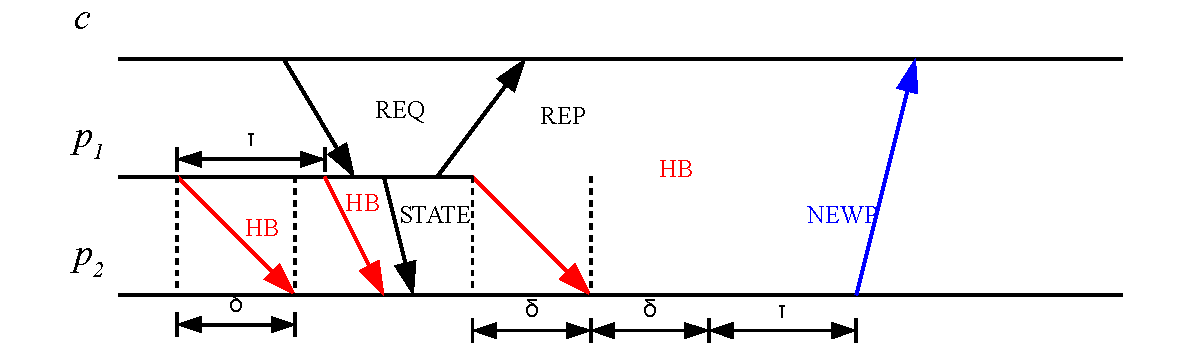
\includegraphics[width=1.0\textwidth]{figs/09/pb1}
\end{figure}

\end{frame}

%-------------------------------------------------------------------------
\begin{frame}{Simple protocol -- Proof of correctness}
	
\BIL
\item[PB2] If a client request arrives at a server that is not the current primary, then the request is ignored
\item[Proof] Trivially follows from the protocol	
\EIL

\end{frame}

%-------------------------------------------------------------------------
\begin{frame}{Simple protocol -- Proof of correctness}
	
\BIL
\item[PB3] There exist fixed values $k$ and $\Delta$ such that the service
behaves like a single $(k, \Delta)$-bofo service
\item[Proof] Find $k$, $\Delta$
\BI
\item At most one process can fail: $k=1$
\item $\Delta = \tau + 4\delta$:
\BI
\item assume $p_1$ crashes at $t_c$
\item any client request sent to $p_1$ at time $t_c - \delta$ or later may be lost
\item $p_2$ may not become the new primary until $t_c + \tau + 2\delta$
\item client may not learn that $p_2$ is new primary for another $\delta$
\EI
\EI
\EIL

\begin{figure}
	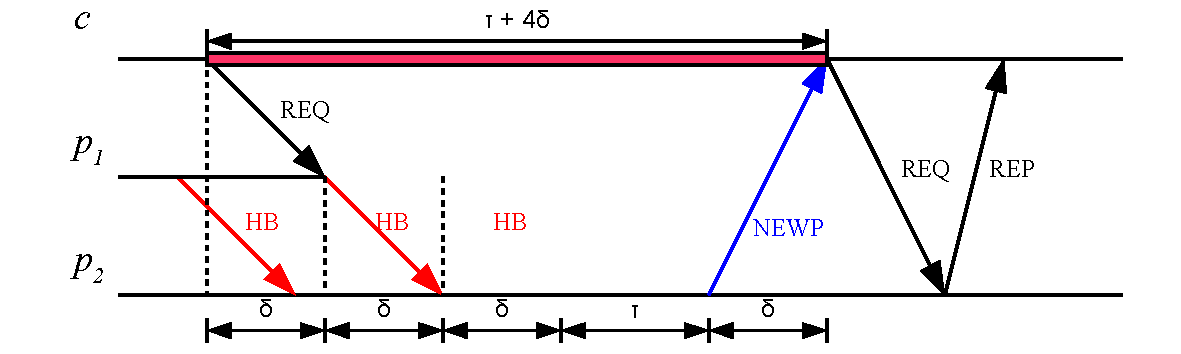
\includegraphics[width=0.9\textwidth]{figs/09/pb2}
\end{figure}

\end{frame}

%-------------------------------------------------------------------------
\begin{frame}{Simple protocol -- Questions}

\begin{block}{Question}	
What kind of consistency model is provided by this simple protocol?
\end{block}

\pause
\bigskip
\begin{block}{Answer: Linearizability}
An execution $E$ is linearizable provided that there exists a sequence (\alert{linearization}) $H$ such that
\BE
\item[L1] $H$ contains exactly the same operations that occur in $E$, each paired with the return value received in $E$
\item[L2] $H$ is a legal history of the sequential data type that is replicated
\item[L3] the total order of operations in $H$ is \alert{compatible} with the real-time partial order $<_{E,rt}$
\EE	
\end{block}

\note{
Given that we are assuming no communication failures, the simple sending
of a message before the crash means that the message will be received,
before the backup actually declare itself as new primary.
}

\end{frame}

%-------------------------------------------------------------------------
\begin{frame}{Primary-backup -- Multiple backups}

\structure{System model}:

\BI
\item point-to-point communication
\item \alert{Perfect Channels}
\item perfect failure detector $P$
\item FIFO channels
\item at most $f < n$ servers crash
\EI

\bigskip
\structure{$n$ servers}:
\BI
\item $p_1, \ldots, p_n$
\EI	

\end{frame}

%-------------------------------------------------------------------------
\begin{frame}[shrink]{Primary-backup -- Multiple backups}

\begin{Procedure}
\caption{Protocol executed by process $p_i$}
\UPON{\RECEIVE $\langle \REQ, \Id, r \rangle$ \FROM $c$}{
  $\Servers \gets \Servers - \{ p_j : p_j \in \Servers \wedge j<i \}$\;
  \If{$\Id \not\in \State$}{
  	$\State \gets \Update(\State, r)$\;
    \SEND $\langle \STATE, \State, \Id \rangle$ \TO $\Servers$\;
    \WAIT $\RECEIVE \langle \ACK, \Id \rangle$ \FROM $\Servers$\;
  }
  \SEND $\langle \REP, \Id, \Reply(r) \rangle$ \TO $c$\;
}	
\BlankLine
\UPON{$\Suspect(p_j)$}{
  $\Servers \gets \Servers - \{ p_j \}$\;
}
\BlankLine
\UPON{\RECEIVE $\langle \STATE, \Id, s \rangle$ \FROM $p_k$}{
  $\Servers \gets \Servers - \{ p_j : p_j \in \Servers \wedge j<k \}$\;
  \If{$p_k \in \Servers$}{
    $\State \gets s$\;
    \SEND $\langle \ACK, \Id \rangle$ \TO $p_k$\;
  }
}
\end{Procedure}

\end{frame}

%-------------------------------------------------------------------------
\begin{frame}[shrink]{Primary-Backup -- Client code}

\begin{Procedure}
\caption{Protocol executed by client $c$}

\UPON{initialization}{
	$\Map\ \Responses \gets \NEW\ \Map()$;
}
\BlankLine
\UPON{\RECEIVE $\langle \REP, \Id, v \rangle$}{
  $\Responses[\Id] \gets v$\;
}
\BlankLine
\UPON{$\Suspect(p_j)$}{
  $\Servers \gets \Servers - \{ p_j \}$\;
}
\BlankLine
\UPON{$\Operation(r)$}{
  $\Id \gets \NewId()$\;
  \While{$\Servers \neq \emptyset$ \OR $\Responses[\Id] = \NIL$}{
    $p_k \gets \mathsf{min}(\Servers)$\;
    \SEND $\langle \REQ, \Id, r \rangle$ \TO $p_k$\;
    \WAIT $\Responses[\Id] \neq \NIL$ \OR $p_k \notin \Servers$\;
  }
  \Return $\Responses[\Id]$\;
}
\end{Procedure}	
	
\end{frame}


%-------------------------------------------------------------------------
\begin{frame}{Primary-backup -- Multiple backups}
	
\BIL
\item How large is the failover time?\\
  \pause \alert{$\tau + 2\delta$}, as before (hidden in the Failure Detector)
\item How large is the outage period $\Delta$?\\
  \pause \alert{$(\tau + 2\delta)f$}
\item What kind of consistency model we obtain if all operations are
  handled by the primary?\\
  \pause \alert{Linearizability}
\item What kind of consistency model we obtain if only write operations
  are handled by the primary?\\
  \pause \alert{Sequential consistency}
\EI	
	
\end{frame}

%-------------------------------------------------------------------------
\begin{frame}{Lower bounds}

\BIL
\item Assuming that no more than $f$ \alert{components} can fail, what are the 
  smallest possible values (\alert{lower bounds}) of 
  \BI
  \item the degree of replication
  \item the failover time?
  \item the blocking time 
  \EI
\item Knowing the lower bounds for a problem enables to evaluate the quality of a protocol
\item Tight lower bounds $\rightarrow$ optimal protocols
\item Components: 
	\BI
	\item Processes
	\item Point-to-point links
\item Up to $f$ crash+link failures $\rightarrow$ at most $f$ processes may
crash or $f$ links may crash or $f_1$ links + $f_2$ processes = $f$ components
	\EI
\EI
\end{frame}

%-------------------------------------------------------------------------
\begin{frame}{Lower bounds}
	
\begin{table}
\begin{tabular}{|c|c|c|c|}
\hline
Failure & Degree of & Blocking & Failover \\
Model & Replication & Time     & Time \\
\hline
crash & $n>f$ & $0$ & $f\delta$ \\
\hline
crash+link & $n > f+1$ & $0$ & $2f\delta$ \\
\hline	
rec-omission & $\left\lfloor \frac{3f}{2} \right\rfloor$ & $2\delta$ & $2f\delta$ \\
\hline
send-omission & $n>f$ & $2\delta$ & $2f\delta$ \\
\hline
omission & $n>2f$ & $2\delta$ & $2f\delta$ \\
\hline
\end{tabular}
\end{table}

\end{frame}

%-------------------------------------------------------------------------
\begin{frame}{Lower bounds}
	
\begin{block}{Crash+link}
To tolerate up to $f$ crash+link failures, more than $f+1$ servers are
needed
\end{block}

\begin{columns}
\begin{column}{0.6\textwidth}
\begin{block}{Proof -- by contradiction}
Suppose $n=f+1$ servers is sufficient
\BI
\item divide the $n$ servers in two subsets $A$ and $B_1 \ldots B_f$
\item if all server in $B$ crash, $A$ must become primary
\item if $A$ crashes, one of servers $B_i$ must become primary
\item what if all $f$ links between $A$ and $B_i$ fails?
\EI
\end{block}
\end{column}
\hfill
\begin{column}{0.30\textwidth}
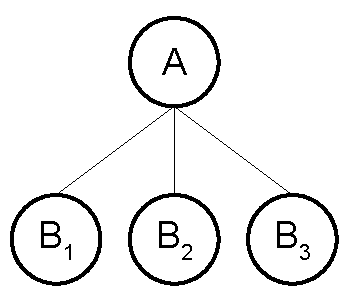
\includegraphics[width=\textwidth]{figs/09/lowerbound}
\end{column}
\end{columns}

\end{frame}

%-------------------------------------------------------------------------
\begin{frame}{Multiple primaries}
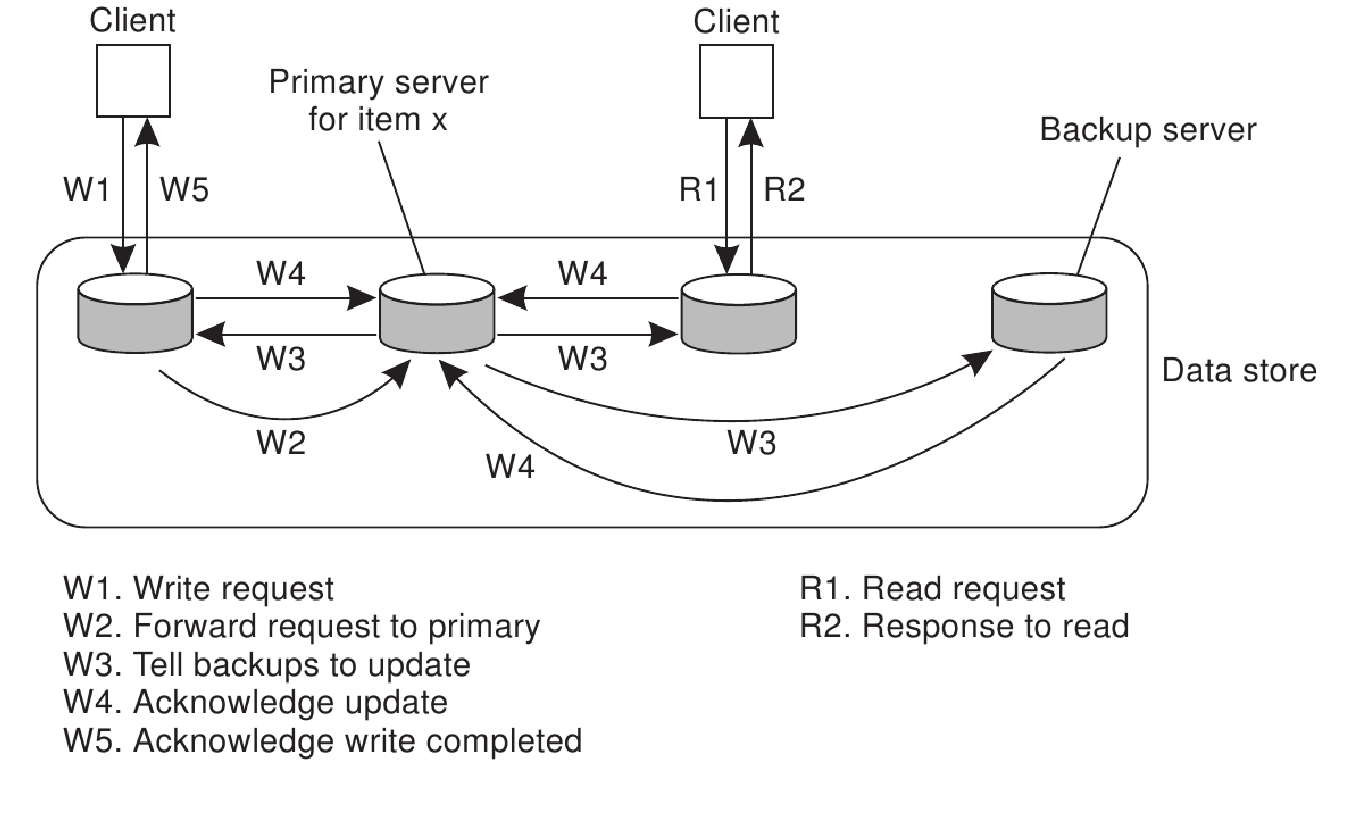
\includegraphics[width=\textwidth]{figs/09/multipleprimary}
\end{frame}

%%%%%%%%%%%%%%%%%%%%%%%%%%%%%%%%%%%%%%%%%%%%%%%%%%%%%%%%%%%%%%%%%%%%%%%%%%
\subsection{Quorum protocols}

%-------------------------------------------------------------------------
\begin{frame}{Quorum protocols (Gifford, 1979)}
	
\begin{definition}
Quorum-based protocols guarantee that each operation is carried out in such
a way that a majority vote (a quorum) is established.
\BI
\item \alert{Write quorum} $n_W$: the number of replicas that need to acknowledge the receipt of the update to complete the update
\item \alert{Read quorum} $n_R$: the number of replicas that are contacted when a data object is accessed through a read operation
\EI
\end{definition}

\smallskip
\structure{Constraints}\\
\BI
\item $n_R + n_W > n$ (prevent R-W conflicts)
\item $n_W > n/2$	  (prevent W-W conflicts)
\EI
% \end{column}	
% \end{columns}	

\smallskip
\structure{The algorithm}\\
\BI
\item To read, the most up-to-date entry is taken
\item Quorums guarantee that the last written entry will be present
\EI

\end{frame}

%-------------------------------------------------------------------------
\begin{frame}{Quorum protocols (Gifford, 1979)}

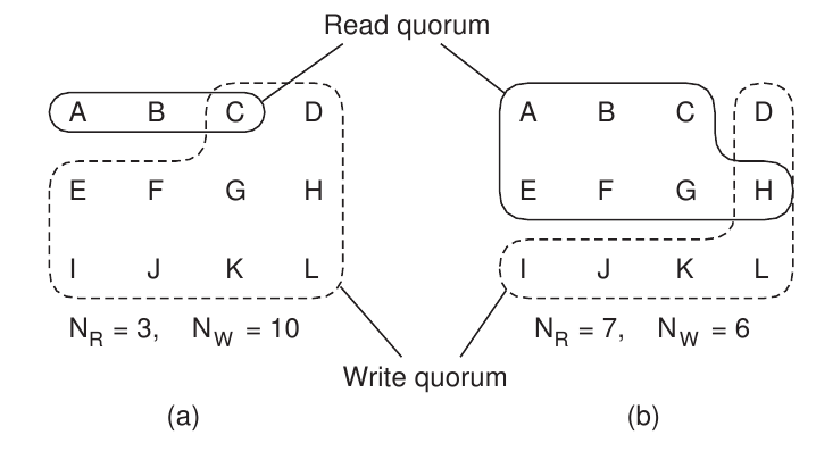
\includegraphics[width=\textwidth]{figs/09/quorum1}

\end{frame}

%-------------------------------------------------------------------------
\begin{frame}{Quorum protocols (Gifford, 1979)}

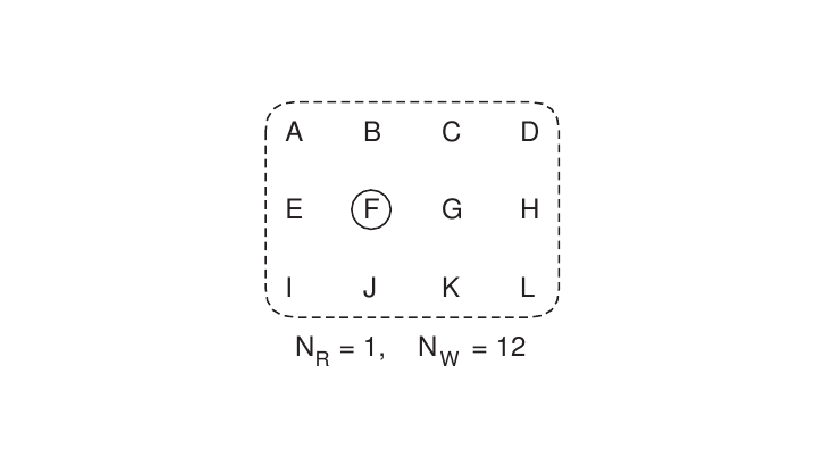
\includegraphics[width=\textwidth]{figs/09/quorum2}

\end{frame}

%%%%%%%%%%%%%%%%%%%%%%%%%%%%%%%%%%%%%%%%%%%%%%%%%%%%%%%%%%%%%%%%%%%%%%%%%%
\subsection{State machines}

%-------------------------------------------------------------------------
\begin{frame}{State machine}

\begin{definition}[State machine]
A \alert{state machine} consists of:
\BI
\item \alert{State variables}
\item \alert{Commands} which transforms its state
  \BI
  \item Implemented by deterministic programs
  \item Atomic with respect to other commands
  \EI
\EI
\end{definition}

\begin{block}{Specification}
\BI
\item \alert{Agreement}: every correct replica receives the same set of
  commands
\item \alert{Order}: every non-faulty state machine processes the commands
  it receives in the same order
\EI
\end{block}

\end{frame}

%-------------------------------------------------------------------------
\begin{frame}[t]{Implementing linearizability -- General scheme}

\structure{Implementation}\\
\BI
\item The initiator A-broadcasts all read, write requests to all servers
\item When the message is A-delivered at the initiator, it replies to the client
\EI

\smallskip
\structure{Correctness}\\
\BI
\item  All replicas execute read, write in the same order
\EI

\smallskip
\structure{Assumptions}\\
\BI
\item Synchronous system
\item Asynchronous system with $\diamond S$ failure detector
\EI

\end{frame}

%-------------------------------------------------------------------------
\begin{frame}[t]{Implementing sequential consistency -- General scheme}

\structure{Implementation}\\
\BI
\item The initiator A-broadcasts write requests to all servers
\item When the message is A-delivered, the replica updates its local copy
\item Read request are replied immediately by the initiator
\EI

\smallskip
\structure{Correctness}\\
\BI
\item Writes are executed in the same order everywhere
\item Reads are consistent with local order
\EI

\smallskip
\structure{Assumptions}\\
\BI
\item Synchronous system
\item Asynchronous system with $\diamond S$ failure detector
\EI

\end{frame}

%-------------------------------------------------------------------------
\begin{frame}[t]{Implementing causal consistency -- General scheme}

\structure{Implementation}\\
\BI
\item The initiator C-broadcasts write requests to all servers
\item When the message is C-delivered, the replica updates its local copy
\item Read request are replied immediately by the initiator
\EI

\smallskip
\structure{Correctness}\\
\BI
\item Writes are executed in a causal order
\item Reads are consistent with local (and causal) order
\EI

\smallskip
\structure{Assumptions}\\
\BI
\item Asynchronous system
\EI

\end{frame}

%-------------------------------------------------------------------------
\begin{frame}{Hypervisor-based fault tolerance}
	
\BIL
\item Implement state machine on \alert{virtual machines} running on the same instruction-set as underlying hardware
\item Undetectable by higher layers of software
\item One of the great come-backs in systems research!
	\BI
	\item CP-67 for IBM 369 [1970]
	\item Xen [SOSP 2003], VMware
	\EI
\item State transition should be deterministic
\item ...but some VM instructions are not (e.g. time-of-day)!
\item Two types of commands
	\BI
	\item Virtual-machine instructions
	\item Virtual-machine interrupts (with DMA input)\\
	Interrupts must be delivered at the same point in cmd sequence
	\EI
\EIL
	
\end{frame}

%-------------------------------------------------------------------------
\begin{frame}{Hypervisor-based fault tolerance}

\BIL
\item Thomas C. Bressoud, Fred B. Schneider. Hypervisor-based Fault Tolerance. ACM TOCS, 14(1):80-107
\item John R. Douceur an Jon Howell. Replicated Virtual Machines.  Microsoft Research TR-2005-119
	\BI
	\item Technical paper associated to a patent
	\EI
\item Brendan Cully et al. Remus: High Availability via Asynchronous Virtual Machine Replication. NSDI'08.
\BI
\item Best paper award
\item Real implementation for XEN
\EI
\EIL

\end{frame}


%%%%%%%%%%%%%%%%%%%%%%%%%%%%%%%%%%%%%%%%%%%%%%%%%%%%%%%%%%%%%%%%%%%%%%%%%%
\subsection{Client-centric consistency}

%-------------------------------------------------------------------------
\begin{frame}{Client-centric consistency - Naive implementations}

\BIL
\item  Each write operation is assigned a unique identifier
\BI
\item Done by the server where the operation is requested
\EI
\item For each client $c$, we keep track of:
  \BI
  \item \alert{Read set $\mathit{WS}_r$}: contains write operations relevant to the read operations performed by $c$
  \item \alert{Write set $\mathit{WS}_w$}: contains write operations relevant to the write operations performed by $c$
  \EI
\item For each server, we keep track of:
  \BI
	\item \alert{Write set $\mathit{WS}$}: contains the write operations executed so far
  \EI
\EIL

\end{frame}

%-------------------------------------------------------------------------
\begin{frame}{Monotonic reads - Naive implementation}

\BIL
\item To perform a read operation $o_r$, a client:
	\BI
	\item send $o_r$ and its read set $\mathit{WS}_r$ to the server
	\EI
\item The server
\BI
\item Checks whether all the writes in $\mathit{WS}_r$ have been executed locally ($\mathit{WS}_r \subseteq \mathit{WS}$?)
\item If not, asks the appropriate servers the missing operations $O$
\item Applies the operations $O$ and add them to $\mathit{WS}$
\item Returns the requested value and the $\mathit{WS}$ set to the client
\EI
\item The client
\BI
\item Adds $\mathit{WS}$ to its local read set: $\mathit{WS}_r = \mathit{WS}_r \cup \mathit{WS}$
\EI
\EIL

\end{frame}

%-------------------------------------------------------------------------
\begin{frame}{Read your writes - Naive implementation}

\BIL
\item To perform a read operation $o_r$, a client:
	\BI
	\item send $o_r$ and its write set $\mathit{WS}_w$ to the server
	\EI
\item The server
\BI
\item Checks whether all the writes in $\mathit{WS}_w$ have been executed locally ($\mathit{WS}_w \subseteq \mathit{WS}$?)
\item If not, asks the appropriate servers the missing operations $O$
\item Applies the operations $O$ and add them to $\mathit{WS}$
\item Returns the requested value to the client
\EI
\item To perform a write operation $o_w$, a client $c$
	\BI
	\item send $o_w$ to the server
	\item add $o_w$ to the write set $\mathit{WS}_w$
	\EI
\EIL

\end{frame}

%%%%%%%%%%%%%%%%%%%%%%%%%%%%%%%%%%%%%%%%%%%%%%%%%%%%%%%%%%%%%%%%%%%%%%%%%%
\section{CAP Theorem}

%-------------------------------------------------------------------------
\begin{frame}{CAP theorem}
	
\begin{theorem}[Impossibility of CAP]	
It is impossible for a web service to provide more than two of the following three guarantees:
\BI
\item \textbf{C}onsistency
\item \textbf{A}vailability
\item \textbf{P}artition-tolerance	
\EI
\end{theorem}

\smallskip
\BIL
\item This is the reason why Amazon Web Services only provide eventual
consistency
	\BI
	\item {\footnotesize \bibentry{eventual-consistent-nonote}}
	\EI 
\item Similar stands have been taken for example by HP
	\BI
	\item {\footnotesize \bibentry{nofreelunchds}}
	\EI
\EI


\end{frame}

%-------------------------------------------------------------------------
\begin{frame}{CAP theorem}

\structure{History}:

\BIL
\item First introduced by Eric Brewer in a keynote at PODC'00
\BI
\item {\footnotesize \bibentry{brewer-cap}}
\EI
\item Formally proved by Gilbert and Lynch two years later
\BI
\item {\footnotesize \bibentry{cap-proof}}
\EI
\EIL
\end{frame}

%%%%%%%%%%%%%%%%%%%%%%%%%%%%%%%%%%%%%%%%%%%%%%%%%%%%%%%%%%%%%%%%%%%%%%%%%%

\section{Bibliography}

%-------------------------------------------------------------------------
\begin{frame}{Reading material}

{\footnotesize
\BIL
\item \bibentry{primarybackup}
\item \bibentry{statemachine}
\EIL
}


\end{frame}

\end{document}